\documentclass[11pt]{article}

% --- Packages ---
\usepackage[usenames, dvipsnames]{color} % Cool colors
\usepackage{enumerate, amsmath, amsthm, amssymb, mathrsfs, algorithm, algpseudocode, fontawesome, pifont, subfig, fullpage, csquotes, dashrule, tikz, bbm, booktabs, bm, hyperref, wasysym}
\usepackage[framemethod=TikZ]{mdframed}
\usepackage[numbers]{natbib}
\usepackage[normalem]{ulem}

% --- Misc. ---
\hbadness=10000 % No "underfull hbox" messages.
\setlength{\parindent}{0pt} % Removes all indentation.

% -- Commands --
% Dynamically sized mid bar.
\newcommand{\bigmid}{\mathrel{\Big|}}

% ---- Colors and Notes ----
% ---- Colors and Notes ----
\definecolor{dblue}{RGB}{98, 140, 190}
\definecolor{dmblue}{RGB}{169, 193, 219}
\definecolor{dlblue}{RGB}{216, 235, 255}
\definecolor{dred}{RGB}{195, 112, 113}
\definecolor{dorange}{RGB}{230, 169, 132}
\definecolor{dgreen}{RGB}{83, 127, 85}
\definecolor{dmgreen}{RGB}{118, 167, 125}
\definecolor{dlgreen}{RGB}{154, 195, 157}
\definecolor{dtan}{RGB}{221, 215, 200}
\definecolor{dpink}{RGB}{207, 166, 208}
\definecolor{dyellow}{RGB}{255, 248, 199}
\definecolor{dgray}{RGB}{46, 49, 49}

% Lights
\definecolor{dlblue}{RGB}{169, 193, 219}
\definecolor{dlgreen}{RGB}{154, 195, 157}
\definecolor{dyellow}{RGB}{246, 240, 223}


% URL
\newcommand{\durl}[1]{\textcolor{dblue}{\underline{\url{#1}}}}
\newcommand{\tx}[1]{\text{#1}}

% Circled Numbers
\newcommand*\circled[1]{\tikz[baseline=(char.base)]{\node[shape=circle,draw,inner sep=0.7pt] (char) {\footnotesize{#1}};}}
% From: http://tex.stackexchange.com/questions/7032/good-way-to-make-textcircled-numbers

% Under set numbered subset of equation
\newcommand{\numeq}[3]{\underset{\textcolor{#2}{\circled{#1}}}{\textcolor{#2}{#3}}}

\newcommand{\dnote}[1]{\textcolor{dblue}{Dave: #1}}

% ---- Abbreviations -----
\newcommand{\tc}[2]{\textcolor{#1}{#2}}
\newcommand{\ubr}[1]{\underbrace{#1}}
\newcommand{\uset}[2]{\underset{#1}{#2}}
\newcommand{\eps}{\varepsilon}
\newcommand{\KL}[2]{D_{\text{KL}}\left(#1 \mid \mid #2\right)}
\newcommand{\bKL}[2]{D_{\text{KL}}\left(#1 \bigmid \bigmid #2\right)}

% Typical limit:
\newcommand{\nlim}{\underset{n \rightarrow \infty}{\lim}}
\newcommand{\nsum}{\sum_{i = 1}^n}
\newcommand{\nprod}{\prod_{i = 1}^n}

% Add an hrule with some space
\newcommand{\spacerule}{\begin{center}\hdashrule{2cm}{1pt}{1pt}\end{center}}

% Mathcal and Mathbb
\newcommand{\mc}[1]{\mathcal{#1}}
\newcommand{\indic}{\mathbbm{1}}
\newcommand{\bE}{\mathbb{E}}

\newcommand{\longra}{\longrightarrow}
\newcommand{\longla}{\longleftarrow}
\newcommand{\ra}{\rightarrow}
\newcommand{\la}{\leftarrow}

% argmin, argmax.
\DeclareMathOperator*{\argmin}{arg\,min}
\DeclareMathOperator*{\argmax}{arg\,max}

% Quick Matrix.
\newcommand{\mat}[1]{\begin{bmatrix}#1\end{bmatrix}}

% ---- Figures, Boxes, Theorems, Etc. ----

% Basic Image
\newcommand{\img}[2]{
\begin{center}
\includegraphics[scale=#2]{#1}
\end{center}}

% Put a fancy box around things.
\newcommand{\dbox}[1]{
\begin{mdframed}[roundcorner=4pt, backgroundcolor=gray!5]
\vspace{1mm}
{#1}
\end{mdframed}
}

%  --- PROOFS ---

% Inner environment for Proofs
\newmdenv[
  topline=false,
  bottomline=false,
  rightline = false,
  leftmargin=10pt,
  rightmargin=0pt,
  innertopmargin=0pt,
  innerbottommargin=0pt
]{innerproof}

% Proof Command
%\newenvironment{dproof}{\begin{proof} \text{\vspace{2mm}} \begin{innerproof}}{\end{innerproof}\end{proof}\vspace{4mm}}
\newenvironment{dproof}[1][Proof]{\begin{proof}[#1] \text{\vspace{2mm}} \begin{innerproof}}{\end{innerproof}\end{proof}\vspace{4mm}}


% Dave Definition
\newcounter{DaveDefCounter}
\setcounter{DaveDefCounter}{1}

\newcommand{\ddef}[2]
{
\begin{mdframed}[roundcorner=1pt, backgroundcolor=white]
\vspace{1mm}
{\bf Definition \theDaveDefCounter} (#1): {\it #2}
\stepcounter{DaveDefCounter}
\end{mdframed}
}

% Block Quote
\newenvironment{dblockquote}[2]{
\begin{blockquote}
#2
\vspace{-2mm}\hspace{10mm}{#1} \\
\end{blockquote}}

% Algorithm
\newenvironment{dalg}[1]
{\begin{algorithm}\caption{#1}\begin{algorithmic}}
{\end{algorithmic}\end{algorithm}}

% Dave Table
\newenvironment{dtable}[1]
{\begin{figure}[h]
\centering
\begin{tabular}{#1}\toprule}
{\bottomrule
\end{tabular}
\end{figure}}

% For numbering the last of an align*
\newcommand\numberthis{\addtocounter{equation}{1}\tag{\theequation}}


\newtheorem{assumption}{Assumption}
\newtheorem{conjecture}{Conjecture}
\newtheorem{corollary}{Corollary}
\newtheorem{claim}{Claim}
\newtheorem{example}{Example}
\newtheorem{lemma}{Lemma}
\newtheorem{proposition}{Proposition}
\newtheorem{remark}{Remark}
\newtheorem{theorem}{Theorem}


% Nice coloring of references.
\usepackage{hyperref}
\hypersetup{               
    colorlinks=true,              
    breaklinks=true,               
    urlcolor=dblue,
    linkcolor=dgreen,
    linkbordercolor=dgreen,
    citecolor=dblue,
    citebordercolor=dblue
}



\title{NeurIPS 2019 Notes \\ \Large{Vancouver, BC, Canada}}
\author{David Abel\footnote{\durl{http://david-abel.github.io}} \\ \durl{david_abel@brown.edu}}
\date{December 2019}

\begin{document}
\maketitle
\tableofcontents
\newpage


This document contains notes I took during the events I managed to make it to at NeurIPS 2019 in Vancouver, BC, Canada. Please feel free to distribute it and shoot me an email at \durl{david_abel@brown.edu} if you find any typos or other items that need correcting. \\

I was in meetings most of the conference this year, so I missed a lot more than usual. \\


\section{Conference Highlights}




% ------------
% -- Monday --
% ------------
% \newpage
% \section{Monday December 9th: Tutorials}
% The first session I made it to is Katja Hoffman's overview talk on RL.

\subsection{Reinforcement Learning: Past, Present, and Future Perspectives by Katja Hofmann}

RL is everywhere in our lives! We make decisions all the time: what socks to wear, what talks to attend, what to eat. But we also make these decisions {\it under uncertainty}. \\

Q: How can we describe how an agent interacts with an environment, collects experience, and learns from those experiences? \\

$\ra$ This is what RL is all about! Highly interdisciplinary---draws from neuroscience and psychology, but today will be focused on computational perspective. \\





% -------------
% -- Tuesday --
% -------------
\newpage
\section{Tuesday December 10th: Main Conference}
The main conference begins!

\subsection{Session: Deep Learning Theory}

First up is the ``Outstanding New Directions" paper on uniform convergence and generalization error in deep learning.

\spacerule
\subsubsection{Outstanding New Directions Paper: Uniform Convergence may be Unable to Explain Generalization in Deep Learning~\cite{nagarajan2019uniform}}

Talk by Vaishnavh Nagarajan. \\

{\bf Question:} Why do over-parameterized networks generalize well? \\


Previous work: bound generalization bound (test error - train error $\leq$ generalization error), but these bounds all come from {\it uniform convergence}. \\

{\bf This paper:} this direction of using uniform convergence to solve the generalization error puzzle may be limited! \\

\ddef{Uniform convergence bounds}{A bound on the generalization gap based on the representational complexity of the whole hypothesis class:
\begin{equation}
    \text{test error} - \text{train error} \leq O\left( \sqrt{\frac{f(\mc{H})}{m}}\right)
\end{equation}}

previously proposed solution; refined uniform convergence bounds, leading to lots of new tools; PAC-Bayes, Rademacher Complexity, Covering Numbers, compression, and so on. \\

But! Each of these bounds:
\begin{enumerate}
    \item Is too large/grow with parameter count.
    \item Or are too small but don't hold on the original network (require change to network).
\end{enumerate}


{\bf First Finding:} these existing generalization bounds {\it increase} with training set size empirically.
\begin{itemize}
    \item Focus has been on parameter count dependence, not training set size.
    \item We need to worry about training-dataset-size too!
\end{itemize}

{\bf Second Finding:} Provable failure of uniform convergence.
\begin{itemize}
    \item There are situations where any uniform convergence bound, however refined, will fail to explain generalization (it will be vacuous).
    \item Main proof idea: {\it tightest uniform convergence}. What is the smallest uniform convergence for a given learner/hypothesis class? Can show even this is vacuous for deep nets.
    
    $\ra$ High level: even most refined hypothesis class is too complex.
\end{itemize}

Setup:
\begin{itemize}
    \item Given a training set $\mc{S}$, algorithm $h_S \in \mc{H}$, then w.h.p. $\mc{S} \sim D$:
    \[
    \text{test-error}(h_S) - \text{train-error}(h_S) \leq \text{generalization gap}
    \]
    
    \item Now, exclude all irrelevant hypothesis leads to the {\it most refined hypothesis class] $\mc{H}^*$}.
    
    \item Proof idea is to show that, in binary (hypersphere) classification, even this most refined class will have vacuous generalization bounds.
    
    \item Learning details: 1000-dimensional hypersphere classification, 1-hidden layer ReLu, 100k units, SGD, trained to zero error.
\end{itemize}


\dbox{{\bf Conclusion:} Can uniform convergence provide a complete answer to the generalization puzzle? We believe {\it it cannot}}

Future Work:
\begin{itemize}
    \item Mathematically characterizes the complexities in the decision boundary of deep networks
    \item Explore other learning theoretic tools such as stability
    \item Need to go beyond uniform convergence to explain generalization in deep nets.
\end{itemize}

\spacerule
\subsubsection{On Exact Computation with an Infinitely Wide Neural Net~\cite{arora2019exact}}

Talk by Rusong Wang. \\

Recent work: shows NNs with sufficiently large width can achieve 0 training error via gradient descent (Li and LLiang, Du et al., Allen-Zhu et al.) \\DAVECITE

This work: relationship between infinite width network and neural tangent kernal (NTK). \\

Questions:
\begin{enumerate}
    \item Can we formally show prediction of NNs is equivalent to NTKs when width is sufficinelty large?
    \item How does NTK perform?
\end{enumerate}

First Contribution:
\begin{theorem}
When width is sufficiently large (poly in data, depth, and $1/\eps$), the predictor learned by applying GD on a NN is $\eps$ close to kernel regression predictor of corresponding NTK.
\end{theorem}

Second Contribution:
\begin{itemize}
    \item Experiments with NTK for CNNs with efficient GPU implementations.
    \item Compare test accuracy of different architectures/modifications of different width to NTK.
    \item Main Observations:
    \begin{enumerate}
        \item Performance of NTK is highly correlated with CNN.
        \item Still a gap between performance of CNN and NTK.
    \end{enumerate}
\end{itemize}

Future Directions;
\begin{itemize}
    \item Understand design of neural net architectures and common techniques in deep learning such as batch norm, residual layers.
    \item Combine NTK with other methods.
\end{itemize}

\spacerule
\subsubsection{Generalization Bounds of SGD for Wide and Deep NNs \cite{cao2019generalization}}

Talk by Yuan Cao.\\

{\bf Previous observation} (see above references): wide nets can achieve zero training error, even when the test error remains large. \\

Questions:
\begin{enumerate}
    \item Why do wide neural nets generalize?
    \item What functions can be learned by wide nets?
\end{enumerate}

Results:
\begin{enumerate}
    \item As long as an NN is wide enough, the generalization error can compete with the best function class in the hypothesis class.
    \item New generalization bounds based on the NTK.
    \item The ``classifiability' of underlying data distribution can be measured by some function of the Gram matrix of the NTK (see Jacot et al).
    DAVECITE
\end{enumerate}

Proof is based on: 1) Deep ReLu nets are almost linear in parameteres in a small neighborhood around initialization, and 2) Loss is Lipschitz continuous and almost convex. \\

$\ra$ This result is applicable to general loss functions. \\

Summary:
\begin{enumerate}
    \item New generalization bounds for wide DNNs that do not increase with network width
    \item A random feature model (NTRF) naturally connext over-parameterized DNNs with NTK
    \item Quantification of classifiability of data.
\end{enumerate}

\spacerule
\subsubsection{Efficient and Accurate Estimation of Lipschits Constants for DNNs \cite{fazlyab2019efficient}}

Talk by Alex Robey. \\

{\bf Main Idea:} Efficiently measure Lipschitz constant in NNs. \\

\ddef{Lipschitz Constant}{The smallest $L_2$ such that:
\begin{equation}
    ||f(x) - f(y)||_2 \leq L_2||x-y||_2\ \forall_{x,y \in \mathbb{R}^2}.
\end{equation}}

$\ra$ Extremely useful in ML for exploiting smoothness/structure in function or data space. Also: a lower Lipschitz constant implies more robustness. \\\\

But! It's NP-Hard to compute in general. So how can we estimate it efficiently?
\begin{itemize}
    \item Simple method: can upper bound lipschitz constant via product or norms, but leads to highly conservative upper bound.
    
    \item {\bf This paper;} transform NN into a family of incrementally quadratically constrained linear Nets (IQCLN).
    
    \item Use optimization techniques (induce a semi-definite program) to give a tight upper bound to the Lipschitz constant of the original net.
\end{itemize}

Q: How does this bound compare to existing bounds in the literature? \\

A: This new estimation is much tighter than existing methods. \\

Also take a close look at adversarial robustness as it relates to Lipschitz constant.

\spacerule
\subsubsection{Regularization Effect of Large Initial Learning Rate~\cite{li2019towards}}

Talk by Colin Wei. \\

{\bf Observation:} Large initial learning rate is crucial for generalization. \\
%Small learning rate eventually 

{\bf This Paper:} Explain this phenomena. \\

$\ra$ LR schedule changes order of learning patterns, which leads to generalization.

\begin{itemize}
    \item Small learning rate quickly memorizes hard to fit class signatures (ignores patterns, harms generalization)
    
    \item Large initial learning rate learns easy to fit patterns first: only memorizes hard to fit patterns after annealing. Learns to use all patterns, helps generalization!
\end{itemize}

Experiment on modified CIFAR10:
\begin{itemize}
    \item Group 1: 20\% examples with hard-to-generalize, easy to fit patterns (hard to generalize because of variations in image).
    \item Group 2: 20\% examples with easy-to-generalize but hard-to-fit patterns (colored patches that identify the class).
    \item Group 3: 60\% examples with both patterns.
    
    \item Finding:
    \begin{itemize}
        \item Small LR: memorizes patch, ignores rest of image
        \item Large LR: ignores patch, only learns after annealing.
    \end{itemize}
    \item Also present proof of this trend in linear classification.
\end{itemize}

\spacerule
\subsubsection{Data-Dependent Sample Complexity for Deep NNs~\cite{wei2019data}}

For those that missed the previous talk, this is also by Colin Wei! :) \\

Q: How do we design principled regularizers for deep models? \\

A1: Principled approach---prove upper bounds on generalization error, regularize the upper bounds empirically. \\

But: bottleneck in prior work. Mostly consider the norms of weight matrices, which lead to pessimistic bounds that are exponential in the net depth. \\

{\bf This Work:} Data-Dependent Generalization Bounds. Add $g(\text{weights}, \text{training data})$ as an explicit regularizer, which shows up in generalization bounds. \\

\begin{theorem}
(informal)
\begin{equation}
    g(\cdot) = \frac{\text{jacobian norm of model w.r.t hidden layers} \times {\text{hidden layer norm}}}{\text{margin} \sqrt{\text{train set size}}}.
\end{equation}
\end{theorem}

Roughly measures stability/Lipschitzness of the network around training examples. \\

Final ingredient to derive the regularizer: penalize squared Jacobian norm in loss. Hidden layer controlled by normalization layers. \\

Conclusion:
\begin{itemize}
    \item Tighter bounds by considering data-dependent properties
    \item Bounds avoid exponential dependence on depth.
    \item Optimizing this bounds improves empirical performance.
\end{itemize}

\spacerule

\subsection{Test of Time: Dual Averaging Method for Stochastic Learning and Online Optimization \cite{xiao2010dual}}

Talk by Lin Xiao. \\

Acknowledge influence from Nesterov: this work was inspired by/extension of \citet{nesterov2009primal}. \\

Exciting time to be in ML/AI! It was exciting in 2009 as well. There was lots of excitement about two topics, the conflict of which led to this paper. They were: 1) Stochastic Gradient Descent and 2) Online convex optimization.. \\

SGD in stochastic optimization:
\begin{equation}
    \min_w \bE_z[f(w, z)],
\end{equation}
or in empirical risk minimization:
\begin{equation}
    \min_w \frac{1}{n} \nsum f(w,z_i),
\end{equation}
Simply means doing gradient based updates. \\

$\ra$ Will also need some basic convergence theory:
\begin{enumerate}
    \item $O(1 / \sqrt{t})$ rate if $f(\cdot, z)$ convex and $\alpha_t \sim t / \sqrt{t}$
    \item $O(1 / t)$ if $f(\cdot, z)$ strongly convex and $\alpha_t \sim 1/t$.
\end{enumerate}

In convex optimization:
\begin{itemize}
    \item Input is a convex set $\mc{S}$
    \item Then, for each round, simply:
    \begin{enumerate}
        \item Predict a vector $w_t \in \mc{S}$
        \item Receive a convex loss function $f_t$, suffer loss $f_t(w_t)$
    \end{enumerate}
    \item Goal is to minimize regret:
    \[
    R_T = \sum_{t=1}^T f_t(w_t) - \min_{w \in\mc{W}}\sum_{t=1}^T f_t(w).
    \]
    \item $R_t = O(\sqrt{T})$ for convex, $O(\ln(T))$ for strongly convex.
    
    \item See more by \citet{duchi2011adaptive}.
\end{itemize}

Another exciting area from 2009: compressed sensing/sparse optimization. \\

$\ra$ Lasso \cite{tibshirani1996regression}!
\begin{equation}
    \min_w \frac{1}{2} ||Xw - y||_2^2,\hspace{6mm} \text{subject to} ||w||_1 \leq \delta.
\end{equation}
Lots of theory and algorithms from the 2000s (interior point methods, proximal gradient methods). \\

Proximal gradient method:
\begin{itemize}
    \item Compositve convex optimization:
    \[
    \min_w f(w) + \psi(w),
    \]
    with $f$ convex and smooth, $\psi$ convex and simple.
    \item Subgradient method;
    \[
    w_{t+1} = w_t - \alpha_t (\nabla f(w_t) +\chi_t).
    \]
    \item Proximal gradient method:
    \[
    w_{t+1} = \argmin_w \left\{f(w_t) + \langle \nabla f(w_t), w-w_t\rangle + \psi(w) + \frac{1}{2\alpha} ||w - w_t||^2\right\},
    \]
    with a constant $\alpha$, achieves $O(1/t)$ convergence.
    
    $\ra$ Equivalent form: forward-backward splitting.
    
    \item Soft-thresholding, where $\psi(w) = \lambda ||w||_1$:
    \begin{align}
        w_{t+1}^(i) &= \text{shrink}\left(w_{t+1/2}^{(i)}, \alpha\lambda\right) \\
        \text{shrink}\left(\omega, \alpha\lambda\right) &- \begin{cases}
        \omega - \alpha\lambda& \omega > \alpha\lambda \\
        0& |\omega| \leq \alpha\lambda \\
        \omega + \alpha\lambda& \omega < -\alpha\lambda \\
        \end{cases}
    \end{align}
\end{itemize}

\dbox{{\bf Motivation} for this paper: {\it how do we put together all three of these techniques?}} \\

$\ra$ SGD/OCO meets sparse optimization! \\

Stochastic subgradient method:
\[
w_{t+1} = w_t - \alpha_t (g_t + \chi_t)
\]
where $g_t = \nabla f(w_t,z_t)$, yields a slow convergence rate of $O(1/\sqrt{t})$. \\

Q: But what about sparsity? \\

A: Sure! Extend proximal gradient method in the stochastic setting, where we replace the gradient with a subgradient. \\

{\bf The Algorithm:} Regularized Dual Averaging (RDA) makes two changes: 1) Replace the single linear approximation with the average of all linear approximations, and 2) quadratic penalty becomes smaller, allowing for larger step sizes. \\

\begin{equation}
    w_{t+1} = \argmin_w \left\{\langle \bar{g}_t, w \rangle + \psi(w) + \frac{\gamma}{\sqrt{t}} \frac{||w - w_0||_2^2}{2}\right\},
\end{equation}
where $\bar{g}_t = \frac{1}{t}\sum_{\tau=1}^t g_\tau$. \\

Can replace $\gamma$ with some parameter $\beta_t$ to penalize depending on aspects of the learning problem. Thus, this is why this is an extension of Nesterov's DA method: $\phi(w) = 0$ or indicator of convex set. \\

$\ra$ Standard theory here: same regret/convergence rate. \\

Experiments on MNIST:
\begin{itemize}
    \item Binary classification on MNIST.
    \item Explore impact of the regularization/penalty term on performance.
    \item Compare SGD, proximal methods, RDA.
\end{itemize}

Further results and extensions:
\begin{itemize}
    \item Later interpretation of RDA from \citet{mcmahan2011follow} that shows some equivalence/relationship to Proximal SGD, FTRL-Proximal.
    \item Further developments: manifold identication \cite{lee2012manifold}, analyze the general and strong convex case.
    \item Other extensions: accelerated version of RDA, RDA-ADMM, distributed, and so on.
    
    \item Adaptive RDA (ADA-RDA)~\cite{duchi2011adaptive}: an adaptive version (variant of AdaGrad) of RDA that is well suited to sparsity.
\end{itemize}

Q: What about nonconvex optimization? \\

A: Very active in recent years due to deep learning. \\

$\ra$ Proximal SGD works with $\ell_1$ regularization. \\

Q: Would variants of RDA work for nonconvex optimization? \\

$\ra$ Promising for sparse CNN \cite{jia2018irda}. Provable convergence with constant step size. \\

Final reflections:
\begin{itemize}
    \item Motivation for RDA remains valid today:
    \begin{enumerate}
        \item we know stochastic gradient online optimization is a mainstay of ML.
        \item But, structured sparsity is essential in scaling, too!
    \end{enumerate} 
    \item Additional challenges today: non-convexity!
    
    $\ra$ Also more complex and structured models today as well.
    
    \item Exciting progress lies ahead.
\end{itemize}

\spacerule



\subsection{Session: Reinforcement Learning}
Next up, RL!

\subsubsection{Causal Confusion in Imitation Learning \cite{de2019causal}}


Talk by Pim de Haan. \\

Imitation learning: powerful mechanism for learning complex behaviors! See: flying drones, grasping fish. \\

$\ra$ Simplest version is behavioral cloning, reduces imitation learning to supervised learning. Just learn to clone the expert exactly. Not perfect, though, since errors from the expert accumulate as we move to states outside the regular state distribution. \\

Q: Does more information mean better performance? \\

A: Let's answer via example. Consider learning to drive where an agent learns to drive and sees the first-person view of driving a car. But, also including a ``break light" can lead to confusion! This is causal confusion. \\

That is: consider two systems; 1) predicts expert action from road view and brake indicator, and 2) predicts expert action from only road view. Turns out the 2nd can be better by avoiding confusion! \\

Control {\bf experiments:}
\begin{itemize}
    \item Add nuisance information to the state to create a confounded state representation.
    
    \item Apply this transformation to Atari, Mountain Car, and MuJoCo---specifically this means drawing (visually) information about the past action onto the screen.
    
    $\ra$ Nuisance is roughly a Pong screen with a big number in the bottom left indicating which action was last taken (and so on for other environments).
    
    \item To solve causal confusion, we need:
    \begin{itemize}
        \item Causal graph of expert
        \item Neural net predictor of action given causes
    \end{itemize}
    \item Phase one: model causal graph as binary vector
    \item Training: 1) randomly sample a causal graph, 2) then mask out nuisance part of the state, 3) feed this into an NN to predict action, 4) NN is fit to a behavioral cloning loss to learn a policy.
\end{itemize}

Q: How do we infer the right causal graph?
\begin{itemize}
    \item Expert demonstrations are insufficient, intervention is necessary
    \item Intervene by executing policies
    \item Score graphs based on additional info.
    \item Two Modes of intervention:
    \begin{enumerate}
        \item Targeted intervention by expert queries.
        \item Targeted intervention by policy execution, given access to some rewards in the environment. Graphs with high rewards become more likely.
    \end{enumerate}
    \item Give upper bounds on performance for both modes, results indicate strong learning performance.
    
    $\ra$ Conclude from the data the algorithm infers a good causal graph.
\end{itemize}

Summary:
\begin{itemize}
    \item Causal confusion happens often in imitation learning
    \item More information in the state can hurt performance by being confusing
    \item Solved in benchmark environments by few targeted interventions.
\end{itemize}


\subsubsection{Imitation Learning from Observations by Minimizing Inverse Dynamics Disagreement}

Talk by Chao Yang. \\

\ddef{Imitation learning}{Given an MDP without $R$ and a set of expert demonstrations, find a policy that mimics expert behavior well.}

Q: What if we don't have {\it action} information in these expert demonstrations? So:
\[
D = \{\tau_1, \ldots, \tau_m\} = \{(s_0, \neg a_0, \s_1, \ldots)\}.
\]
Taking the divergence minimization perspective seems feasible (as in GAIL), but generalize state to observation, yields GAiFO. Without actions, though, need anothher trick. So idea for the new loss function is:
\[
\tx{IDD} = \tx{GAIL} -\tx{GAIfO}.
\]

% Overall objective, then is:
% \begin{equation}
%       \min_\pi D-f(\rho_\pi(s,s')|| \rho_E(s,s'))
% \end{equation}

Carry out quantitative comparison to other imitation learning approaches in OpenAI gym environments, achieve state of the art. \\

\subsubsection{Learning to Control Self-Assembling Morpholgies}

Talk by Deepak Pathel. \\

Q: How do we train a robot? \\

A: Lots of options! Demonstrations, batch of data, from scratch/exploration, self-supervision, and so on. \\

$\ra$ But, doing learning from scratch can be challenging for {\it hardware} reasons. Hardware is designed for learned systems, typically, not to make learning to control easy. \\

{\bf Main Idea;} Co-Evolution of control and morphology. \\

Example: A cylinder and a cone can be combined via a magnet to make more complex objects. Individual items are ``dumb" and can't do much, but when they assemble they can create complicated structures. Thus it's about learning to combine (learn to stand up). \\

Q: How do we learn compositional controllers? \\

A: Each limb/component is a separate policy network with shared parameters. Treat these policies as Lego blocks. Let them pass messages to each other and accept messages from others. \\

$\ra$ This idea of message passing we call ``Dynamic Graph Networks". \\

Experiments: 1) combine a large number of mini components (in 3d mujoco like environment) via magnets to get them to stand up, 2) also look at locomotion tasks involving climbing stairs and crossing trenches.


\subsubsection{A Structured Prediction Approach for Generalization in Cooperative Multi-Agent RL \cite{carion2019structured}}

Talk by Nicolas Carion. \\

Setting: lots of agents that must coordinate to solve a task. Each agent is given its own task. \\

{\bf Main contribution:} Find policies that generalize to new agent-task pairs not seeing during training. \\

Idea: compute score on previous pairs, using structured inference, use this to infer new policy on new pairs. \\

Q: How can we increase collaboration across agents? \\

A: Add a new constraint to the optimization to make it a linear program. The constraint encourages agents to cooperate. Further extend the LP to a quadratic program. \\

Experiments in Starcraft: strategy learns to focus attack of an army on a handful units, and thereby seems to encourage cooperation. Also generalizes to new and larger armies. \\

{\bf Conclusion:} A practical method for scaling MARL by generalizing to large instances from small training scenarios.

\subsubsection{Learning Compositional neural Programs with Recursive Tree Search \cite{carion2019structured}}

Talk by Thomas Pierrot. \\

Natural way to define rewards is {\it binary}: did the RL agent succeed or not? \\

$\ra$ But, of course, this makes exploration extremely hard, as the agent only gets feedback after a success. \\

{\bf New agent:} AlphaNPI that uses modularity, hierarchy, and recursion as structural biases to reduce sample complexity, improve generalization, and increase interpretability. \\

Assumptions:
\begin{itemize}
    \item Assumes a hierarchical program specification
    \item Sparse rewards: 1 when the program execution satisifes the spec, and 0 otherwise.
\end{itemize}

AlphaNPI is based on the Neural Program Interpreter: a recursive compositional neural network's policy and a value function estimator. \\

AlphaNPI works as a standard program execution in a computer: execution is saved into a stack, execution is passed back after a subprocedure finishes, and so on.\\

Experiments: AlphaNPI to learn libraries of programs to achieve sorting and searching tasks, seems to work!


\subsubsection{Guided Meta-Policy Search}

Talk by Russell Mendonca. \\

RL has high sample complexity: typical benchmark tasks with SOTA approaches takes on the order of millions of samples required. \\

Meta-Learning is one possible solution to this problem by making efficent use of previous training tasks. \\

$\ra$ But, most meta-RL methods also requires huge amounts of data for the training phase, even if the adaptation is efficient. Also shortcomings in exploration and credit assignment during the training phase. \\

Introduce: Guided Meta-Policy Search, that can quickly adapt to solve any task from the distribution of training tasks.
\begin{itemize}
    \item On each train task, learn a local policy using sample efficient methods.\footnote{\dnote{?}}
    \item Then, using a supervised meta-RL objective, form updated policies. This decouples the meta-RL problem, allowing for the use of off-policy learning.
\end{itemize}

Experimental evaluation in 1) simulated sawyer robot tasks, and 2) ant Locomotion tasks. Method achieves extremely sample efficient learning on these tasks. \\

$\ra$ Also study Meta-learning from demos. \\

Code: \durl{https://github.com/russellmendonca/GMPS}

\subsubsection{Using a Logarithmic Mapping to Enable a Lower Discount Factor \cite{van2019using}}

Talk by Harm ven Seijen. \\

Q: How do we measure performance? \\

A: A few methods:
\begin{align}
    \text{finite horizon} &= \sum_{i=1}^H R_i, \\
    \text{infinite horizon} &= \sum_{i=1}^\infty \gamma^{i-1} R_i,
\end{align}
for $\gamma \in [0,1)$. But, most $\gamma$s need to be near one to be useful/meaningful, which makes learning hard! How can we get around this? \\

Suppose we do linear function approximation with tile coding on a long chain problem
\begin{itemize}
    \item For high discount factors, performance is okay!
    \item For anything below a high discount factor, however, performance is dreadful. Even with more data, even with tuning the tile coding, performance is really bad.
\end{itemize}

Q: But why? \\

A: One idea is to look at the {\it action gap}.

\ddef{Action Gap}{The action gap of a state is:
\begin{equation}
    \Delta_A(s) := Q^*(s,a^*) - Q^*(s,\tilde{a}),
\end{equation}
where $\tilde{a}$ is the best non-optimal action.}

The action gap is useful because it tells us how small our error should be if we want to be optimal. \\

$\ra$ Action gap exponentially decreases the further you get away from positive reward (in a long chain problem). Thus, with small discount factors, this gap will decrease much more rapidly. \\

Q: But why bad behavior for low discount factors? \\

A: Systematiclly disproved lots of hypotheses, but found hypothesis that seemed promising:

(Possible) Cause of bad behavior for low discount factors: {\it poor performance of low discount factors is caused by large size differences in the action gap across the state space}. \\

$\ra$ Gives rise to logarithmic mapping of the discount factor. So: $\tilde{Q} \mapsto \ln(Q)$. \\

{\bf New Algorithm:} (special case with $R \in \mathbb{R})_{\geq 0}$ and deterministic $T$). Logarithmic Q-Learning. Performs Q update where:
    \begin{equation}
        \tilde{Q}_{t+1}(s_t,a_t) := (1-\alpha)\tilde{Q}_t(s_t,a_t) + \alpha f(r_t + \gamma \max_{a'} f^{-1}(\tidle{Q}_t(s_{t+1}, a')).
    \end{equation}
    
Issues in extending to Stochastic Environments. Becuase of Jensen's Inequality ($\bE[\ln(X)] \leq \ln(\bE[X])$, where $X$ is some random variable, so it seems like previous update rule is applied to stochastic environment, converges to underestimate. \\

But! Can be fixed. New update involves two step sizes, one for the ``regular" Q space, one for the logarithmic space. 

\begin{theorem}
This variant of logarithmic Q-learning preserves convergence guarantees of Q-Learning.
\end{theorem}

Empirical performance is good, too: applied to tabular MDPs and propose logDQN; on average it improves over DQN. \\

$\ra$ Underperforms relative to DQN on a few games where the action gaps are too homogeneous.


\subsubsection{Better Exploration with Optimistic Actor Critic}

Talk by Kamil Ciosek. \\

Greedy is bad! \\

But, policy gradients are greedy. Also: use a lower bound on the critic. If the bootstrap is too large, then the value estimate becomes too large, which is amplified by policy optimization. \\

$\ra$ Conservative update reduces overestimation (as in Double Q). \\

Note: combination of greediness + lower bound can lead to pessimistic exploration. Variance is small, don't explore enough. \\

{\bf This Paper:} Use the bootstrap to make an upper bound to achieve optimistic exploration. \\

$\ra$ UCB style exploration bonus. \\

Want a policy that: 1) is close to target policy, and 2) maximizes the critic upper bound. \\

Super easy to implement this form of optimistic exploration: shift the exploration policy in the direction of the upper bound. Empirical results are very promising, improve over Soft Actor-Critic (SAC). 

\subsubsection{Robust Exploration in Oriented-Exploration in LQ Control}

Talk by Hakan Hjalmarsson. \\

{\bf Goal:} Do exploration that is 1) robust and 2) targeted.
\begin{itemize}
    \item Robust: does not destabilize the system or cause failure.
    \item Targeted: provides knowledge that helps complete the task.
\end{itemize}

Handle the exploration-exploitation tradeoff by formulating policy search as a convex optimization problem which can be solved for the global optimum. \\

$\ra$ Focus on Linear Quadratic Control. Task is to find a state-feedback controller to minimize a quadratic cost. \\

Key quantity: the empirical covariance $D = \sum_{t=0}^T \mat{x_t \\ u_t} \mat{x_t \\ u_t}^\top$. \\

Yields a simplified optimization problem. Preserves structure by working with this empirical covariance matrix $D$. \\

Empirical findings: performance of this method is better even though absolute uncertainty is larger. \\

\subsubsection{Tight Regret bounds for Model-Based RL with Greedy Policies}

Talk by Yonathon Efroni. \\

{\bf One Line Summary:} Same minimax bounds to model-based RL with short-term and long-term planning. \\

$\ra$ Factor of $\mc{S}$ less computation. \\

Previous regret bounds;
\begin{itemize}
    \item Model-Based RL: minimax regret $O(\sqrt{HSAT})$
    \item Model-Free RL: Q-Learning regret $O(\sqrt{H^3SAT})$
\end{itemize}

Q: So, why aren't we using model-based RL? \\

A1: Lots of space complexity. \\
A2: High computational complexity (requires MDP solving each episode). \\

This work; model-based RL with short-term planning is minimax optimal for finite-horizon MDPs. \\

Open question: if one-step planning is minimax optimal, why do we need to use lookahead policies?

\subsubsection{Hindsight Credit Assignment}

Talk by Anna Harutyunyan. \\

Central Q of Credit Assignment: How did past actions influence future outcomes? \\

Usual Answer/algorithmic strategy: rely on MDP structure and use {\it time} as main proxy for credit relevance. \\

Example; Credit Assignmeint in RL (CARL) has to figure out what caused him to be wet during the day. As an RL algorithm, CARL would spend many days getting wet by not bringing an umbrella. \\

$\ra$ This paper: try to learn credit relevance {\it explicitly}. \\

Idea: study $P(a \mid x, f(\tau))$, where $a$ is a past action and $f(\tau)$ is some relevant future outcome (like CARL getting rained on). \\

Hindsight Credit Assignment is about rewriting our usual value function:
\begin{equation}
    Q^\pi(x,a) = r(x,a) + \bE_{\tau \sim T(x,\pi)} \left[\sum_{k \geq 1} \gamma^k \frac{P(a \mid x, f(\tau))}{f(\tau)}V^\pi(x')\right].
\end{equation}

Whole new family of algorithms dedicated to learning the hindsight distribution.

\subsubsection{Weight Agnostic Neural Networks}

Talk by Adam Gaier. \\

Central Q of this work: To what extent can neural net architectures alone encode solutions to tasks? \\

$\ra$ A different kind of neural architecture search.
\begin{itemize}
    \item Search for networks that perform without training! Do zero shot learning
    \item But, add single shared weight value used for all connections.
\end{itemize}

Four key steps
\begin{enumerate}
    \item Initiatlize: create pop of minimal nets
    \item Evaluate: test with range of shared wieght values
    \item Rank: by performance/complexity
    \item Vary networks
\end{enumerate}

Test WANNs on a variety of RL tasks (cart pole, bipedal walker, : find that WANNS perform well with and without training, but perhaps more importantly can do so with significantly smaller neural nets. \\

For fun: tried on MNIST as well using the same rough scheme. Random weight finds 82\% accuracy, tuned gets around 92\%. \\

Point: steps toward a new kind of neural architecture search.

Code and more at \durl{weightagnostic.github.io}.



% ------------
% -- Wednesday --
% ------------
\newpage
\section{Wednesday December 11th: Main Conference}
Day two! 

\subsection{Session: Reinforcement Learning}

Mostly in the RL sessions today.

\subsubsection{A Neurally Plausible Model Learns Successor Representations in Partially Observable Environments \cite{vertes2019neurally}}

Talk by Eszter Vertes. \\

Q: How should we represent belief states? \\

A:  Distributed distributional code (DDC), and successor features (SFs)! \\

{\bf This Paper:} How to elegantly combine DDC and SFs to form distributional successor features, how to learn them, and connections to neuroscience. \\

\ddef{Successor representation}{The successor representation is given by:
\[
M^{\pi}(s_i, s_j) = \bE_\pi \left[\sum_{k=0}^\infty \gamma^k \indic\{s_{t+k} = s_j \} \mid s_t = s_i\right].
\]}

% \ddef{Distributed distributional code}{The DDC is given by:
% \[
% \mu_t(o_1, o_2, \ldots, o_t) = \bE_{q(s_t \mid o_1, \ldots, o_t)}[\psi(s_t)],
% \]
% with $\psi(s)$ a vector 
% }

% Distributional successor features:
% \[
% %DDC belief states:
% \mu = \bE[\psi(s)]
% \]
% \[
% % Distr. SFs
% M^{\pi}(\mu) = \bE_\pi
% \]

Q: How do we learn distributional successor features? \\

A: Two problems: 1) update belief states $\mu$, and 2) Learn/compute distributional SFs $M^{\pi}(\mu)$. \\

To learn the distributional SF: three methods
\begin{enumerate}
    \item Online learning: TD Learning using DDC believe states
    \item Offline learning: TD learning using simulations in latent space 
    \item Direct computation: using recurrent network dynamics.
\end{enumerate}

Contributions:
\begin{itemize}
    \item Generalize SFs to POMDPs by exploiting the relationship between DDC belief states and SFs
    \item Propose learning algorithms that span the space of model-free to model-based algorithms with biological plausibility.
    \item Highlight further connections to neuroscience data:
    \begin{itemize}
        \item Propose a novel role of hippocampal replay for learning to infer spatial location
        \item Connects threads in dopamine signals and sensory prediction errors.
    \end{itemize}
\end{itemize}

\spacerule
\subsubsection{DualDICE: Behavior-Agnostic Estimation of Discounted Stationary Distribution Corrections \cite{nachum2019dualdice}}

Talk by Ofir Nachum. \\

{\bf Central Q of the paper:} Off-policy estimation (``if I run this policy, what is the average discounted reward I will get?"). \\

$\ra$ Off-policy makes it tricky! Only get data from some other policy, may not even know which policy was followed. \\

Main Ideas:
\begin{enumerate}
    \item Reduce the off-policy estimation problem to density ratio estimation:
    \[
    d^\pi(s,a) := (1-\gamma) \sum_{t=0}
    \]
    \begin{itemize}
        \item Using importance weighting trick with a finite dataset, can compute the weighted average of the importance weights.
        \item Thus: reduces to the density ratio problem.
    \end{itemize}
    \item DualDICE operator is a zero-reward Bellman operator:
    \[
    B_\pi v(s,a) := \gamma \bE_{s' \sim T, a \sim \pi}[v(s',a)]
    \]
\end{enumerate}

The DualDICE operator then leads to a new error term that consist of minimizing squared Bellman error while also maximizing initial $\nu$-values. Desirable because objective is based on expectations from things we have access to.

\spacerule
\subsubsection{VIREL: A Variational Inference Framework for RL \cite{fellows2019virel}}

Talk by Matthew Fellows. \\

Goal; cast RL as a problem of probaltistic inference. \\

$\fa$ But: existing methods present several theoretical and practical barriers. \\

Two classical approaches:
\begin{enumerate}
    \item Pseudo-likelihood methods, which promote risk-seeking behavior
    \item Maximum entropy RL objective (Soft Actor-Critic), but optimal deterministic policies are not learned, and counterexamples show several cases when optimal RL policy can't be recovered (new result in this paper).
\end{enumerate}

Thus, new desiderata for an inference framework:
\begin{enumerate}
    \item Naturally learns optimal deterministic policies
    \item Temperature not a hyperparameter.
    \item Function approx explicitly used.
    \item Stochastic policies used for learning.
    \item Discounting easily incorporated.
    \item Optimizes the reverse form of KL divergence.
\end{enumerate}

$\implies$ Main result from the work is to outline the VIREL framework, which they show satisfies these desiderata. \\

Yields new class of Actor-Critic algorithms based on Expectation-Maximization. Evaluate on MuJoCo environments and find gains in sample efficiency.

\spacerule
\subsubsection{Unsupervised Curriculua for Visual Meta RL \cite{jabri2019unsupervised}}
% 
Talk by Kyle Hsu. \\

Objective: move RL from highly specialized learning to more general learning. \\

$\ra$ Setting is Meta-RL, in which the policy must also learn to identify the task it's in. \\

{\bf Key Component for Meta-RL;} Task distribution chosen for training in Meta-RL. \\

Q: Can we learn useful Meta-RL strategies by learning from tasks that care chosen without supervision?

A: Yes! This paper: meta-pre-training. Do unserupvised pre-training, then train. \\

Prior work: do task acquisition, then do meta-learning based on the chosen tasks. \\

This Paper; Do these two things jointly to provide an automatic curriculum. \\

Criteria for task distribution; 1) Diverse tasks, and 2) Structure in tasks. Need to trade-off between these two! Use mutual information maximization:
\[
\max_{\theta, \phi} I(\tau; z),
\]
Via an EM like approach: (E-step) updates task distribution, (M-step) do meta-training by updating policy. \\

Q: What kinds of tasks are discovered by the procedure? \\

A: Experiments in VizDoom, visualize different generated tasks. \\

\spacerule
\subsubsection{Policy Continuation with Hindsight Inverse Dynamics \cite{sun2019policy}}

Talk by Hao Sun. \\

Focus: goal-oriented reward sparse tasks. \\

$\ra$ Purely random exploration is clearly impractical due to the sparsity of the reward. But: people learn from failures, not just success! How can we leverage this idea? \\

Two ideas;
\begin{itemize}
    \item One approach: hindsight experience replay (HER) \cite{andrychowicz2017hindsight}, which explicitly tries to learn from failures.
    \item Extrapolating from success! How can we generalize from cases we were successful?
\end{itemize}

New Idea: equip inverse dynamics with hindsight (HID). But, 1-step HID is not enough, so use multi-step policy continuation to achieve multi-step optimality. \\

Experiments on simulated robot domain and grid navigation.

\spacerule
\subsubsection{Learning Reward Machines for Partially Observable RL \cite{icarte2019learning}}

Talk by Rodrigo Icarte. \\

{\bf Main Q:} How can we learn a reward machine from experience? \\

Reward Machines (RMs) are automate based reward functions, extremely useful for specifying complex behaviors. \\


This paper:
\begin{itemize}
    \item Show how to learn RMs from experience (new algorithm: LRM).
    \item Use RMs as memory for partially observable RL
    \item Extends QRMs to work under partial observability
    \item Provide theoretical and empirical analysis of LRM.
\end{itemize}

\begin{figure}[h!]
    \centering
    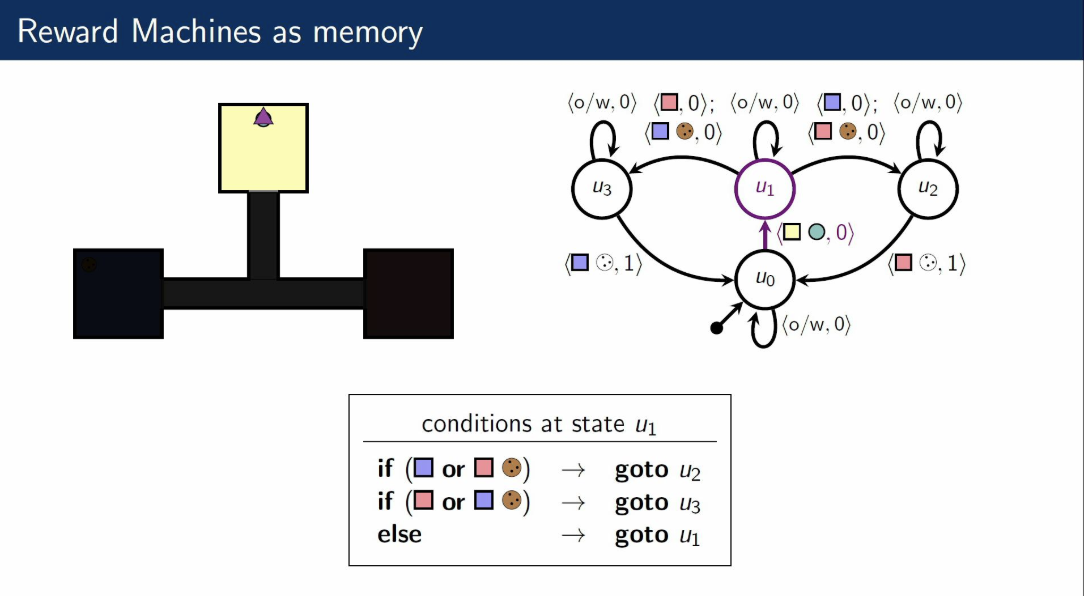
\includegraphics[width=0.7\textwidth]{figures/rm.png}
    \caption{Reward Machines as memory}
    \label{fig:rm}
\end{figure}
 
Introduce RM-DQN, a DQN variant that learns and uses a reward machine. \\

Overall approach:
\begin{itemize}
    \item Collect traces of experience
    \item Do optimization from this experience to propose a candidate RM
    \item Use the candidate RM to train an RL agent
    \item Add extra traces from new RL agent if the RM isn't perfect.
\end{itemize}

\spacerule


\subsection{Keynote: Yoshua Bengio on System 1 and System 2 in Deep Learning}

State of deep learning: amazing progress this century! \\

Q: is it enough to grow datasets, model sizes. or computer speed? \\

Q: Are wwe still far from human-level AI? \\

Some Answers: Narrow AI, sample efficiency, human-provided labels, robustness, stupid errors. Next step could be completely different from deep learning. \\

{\bf Focus Today:} There is a path from deep learning today to system 2! \\


Inspiration: ``Thinking Fast and Slow" by Daniel Kahneman.

\ddef{System 1}{Intuitive, fast unconscious non-linguistic, and habitual decision making/inference.}

Note: deep learning is good at this (system 1)!  

\ddef{System 2}{Slow, logical, sequential, conscious, linguistic, algorithmic,decision making.}

$\implies$ Claim: the future of deep learning is extending what works in system 1 to system 2. \\

Some things that are missing from deep learning right now:
\begin{enumerate}
    \item Out of distribution generalization and transfer
    \item High level cognition: need to move from system 1 to system 2.
    \begin{itemize}
        \item High level semantic representation.
        \item Compositionality.
        \item Causality.
    \end{itemize}
    \item Agent perspective:
    \begin{itemize}
        \item Machines that understand the world by building world models
        \item Knowledge-seeking
    \end{itemize}
\end{enumerate}

{\bf Theme Today:} These three areas are intimately connected, and these connections can help us identify a path forward in AI/ML research. \\

The talk:
\begin{enumerate}
    \item ML Goal: Handle Changes in Distribution
    \item System 2 Basics:  Attention and Consciousness
    \item Consciousness Prior:  Sparse Factor Graph
    \item Theoretical  framework:  meta-learning,  localized  change hypothesis→causal discovery
    \item  Compositional DL architectures
\end{enumerate}

% Consciousness Funtionalities: Roadmap for Priors Empowering System 2
\spacerule
\subsubsection{ML Goal: Handle Changes in Distribution}

Classical ML theory is {\it for i.i.d. data}. Without this assumption we can't say anything about generalization. \\

$\ra$ Naturally, this assumption is unrealistic. \\

But: {\it ``Nature does not shuffle the data, we shouldn't"}
-- Leon Bottou (ICML 2019 Keynote). \\

Out of distribution generalization and transfer breaks the i.i.d. hypothesis, so what do we do? Can we replace it with something else? \\

A: Agent learning needs out-of-distribution (OOD) generalization. \\


Why? Well: Agents face non-stationarities resulting from 1) their actions, 2) actions of other agents, 3) different places, times, sensors, and so on. \\

{\bf Claim:} compositionality helps OOD generalization. \\

$\ra$ Different forms of compositionality, each comes ith different exponential advantages. See, for instance:
\begin{itemize}
    \item Distributed representations
    \item Composition of layers in deep nets DAVEEITE: Montufar NeurIPS 2014
    \item Systematic generalization in language, analogies, abstract reasoning.
\end{itemize}

Q: So, how do we do systematic generalization? \\

A: Important to dynamically recombing existing concepts, {\it even when new combinations have 0 probability under training distributions}. Think of a science fiction scenario! We don't live that, but can still imagine it and draw meaningful insights from it. \\

$\ra$ Current methods are not effective for this. \\

Q: How does what you are proposing contrast with the symbolic AI program? \\

A: Avoids pitfalls of classical AI rule-based symbol manipulation. That is, we need the following:
\begin{itemize}
    \item Need efficient large-scale learning
    \item Need semantic grounding in system 1
    \item Need distributed representations for generalization
    \item Need efficient (trained) search for both systems
    \item Need systems that can properly handle uncertainty in the world.
\end{itemize}

But, we also want:
\begin{itemize}
    \item Systematic generalization
    \item Factorizing knowledge in small exchangeable pieces
    \item manipulating variables, instances, references, and indirection.
\end{itemize}


\spacerule
\subsubsection{System 2 Basics: Attention and Consciousness}

{\bf Claim:} Key ingredient for consciousness is {\it attention}. \\

Q: What is attention? \\

A: Focus on one or a few elements at a time. Content-based soft attention is convenient because we can backprop to learn where to attend. Lots of benefits:
\begin{enumerate}
    \item Neural Machine Translation revolution \cite{bahdanau2014neural}.
    \item SOTA in NLP, self attention/transformers
    \item Memory-extended neural nets
    \item Address vanishing gradients
    \item Operating on unordered sets.
\end{enumerate}

$\ra$ Attention creates a {\it dynamic} connection between two layers of a neural net. \\

From Attention to Consciousness:
\begin{itemize}
    \item ``C"-word is not taboo anymore in cognitive neuroscience
    \item One main theory: ``Global Workspace Theory" \cite{baars2005global}.
    \begin{itemize}
        \item Bottleneck of conscious processing
        \item Selected item is broadcast, stored in short-term memory, conditions perception and action
        \item System 2 like sequential processing, conscious reasoning and planning and imagination.
    \end{itemize}
\end{itemize}

Q: So how can we connect these ideas to machine learning? (can the two communities help each other?) \\

A: ML can help us formalize, in a mechanistic way, and test specific hypothesized functionalities of consciousness. This could: 1) get the magic out of consciousness, 2) understand evolutionary advantage of consciousness by grounding it to computation and statistics. \\

Concsciousness closely related to language: we assign consciousness from humans reporting, and moreover, high level representations are deeply connected to language. \\

$\ra$ Thus, a connection between System 1 and System 2: meaning anchored in low-level perception and action. \\

So need {\it grounded language learning}, such as BabyAI \cite{chevalier2018babyai}.

\spacerule
\subsubsection{Consciousness Prior: Sparse Factor Graph}

Q: So what kinds of priors and structures can we use to get our learning algorithms to use these kinds of abilities? \\

Proposal one: the consciousness prior \cite{bengio2017consciousness}.
\begin{itemize}
    \item Attention: to form conscious state and thought
    \item A thought is a low-dimensional object, few selected aspects of the unconscious state
    \item Need 2 high level states: 1) large unconscious state, and 2) tiny conscious state.
    \item Part of inference mechanism with respct to joint distribution of high-level variables.
\end{itemize}

Concretely, the consciousness prior proposes a {\it sparse factor graph}, where nodes are variables, and edges represent relations between these variables.\\

Why is this a reasonable hypothesis?
\begin{itemize}
    \item Property og high-level variables which we manipulate with language; we can predict {\it some} given very few others.
    
    For instance: ``if I drop the ball, it will fall on the ground"
    
    \item Disentangled factors are not marginally independent (ball, hand, etc)
    \item Prior: sparse factor graph imposes a joint distribution between high-level variables.
    
    \item Note: this prior does not work in the space of pixels.
\end{itemize}


% idea:
% \[
% P(V) \propto \Prod_k \phi_k(V_{sk})
% \]


\spacerule
\subsubsection{Theoretical framework: meta-learning, localized change hypothesis $\ra$ causal discovery}

Meta-Learning (or ``learning to learn"): having multiple time scales of learning.
\begin{itemize}
    \item Bi-level optimization:
    \begin{itemize}
        \item Inner Loop of learning that outputs a loss
        \item Outer loop: continual learning that optimizes the loss from the inner loop
    \end{itemize}
    \item Examples: evolution \& individual learning, Lifelong learning and adaptation to new environments.
\end{itemize}

Q: what causes changes in distribution? \\

{\bf Hypothesis to replace i.i.d. assumption:} the ``localized change hypothesis":

\ddef{Localized Change Hypothesis}{``changes are consequences of an intervention on a few causes or mechanisms." \cite{scholkopf2012causal}}

Then: use OOD generalization as a training signal for factorizing knowledge \cite{bengio2019meta}.
\begin{itemize}
    \item A meta-transfer objective for learning to disentangle causal mechanisms
    \item Learning whether A causes B or vice-versa
    \item Learning to disentangle (A,B) from (X,Y)
    \item Exploit changes in distribution and speed of adaptation to guess causal direction.
\end{itemize}

Newer work: Learning neural causal models from unknown interventions \cite{ke2019learning}. \\

$\ra$ Learning small causal graphs to avoid exponential explosion of number of graphs by parameterizing factorized distribution over graphs. \\

Note: attacking this problem in a very deep learning friendly way. Can plug into the deep learning tools that work already.



\spacerule
\subsubsection{Compositional DL architectures}



Recurrent Independent Mechanisms (RIMs) \cite{goyal2019recurrent}: modularize computation and operate on sets of named and typed objects.
\begin{itemize}
    \item multiple recurrent sparsely interacting modules, each with dynamics and object input-outputs
    \item Results: much better OOD generalization!
    \item Also RIMs as a replacement for LSTM in PPO, find improvements in Atari.
\end{itemize}



Summary: Hypotheses for Conscious Processing by Agents, Systematic Generalization:
\begin{itemize}
    \item Sparse factor graph in space of high-level semantic variables
    \item Semantic variables are causal: agents, intentions, controllable objects
    \item Shared rules across instance tuples
    \item Distributional changes from localized causal interventions.
    
    $\ra$ Changes are mostly localized {\it if you represent things in the right space}
    
    \item Things that are preserved across changes in distribution are the fundamental stable aspects of the world. Meaning should target these aspects.
\end{itemize}

Conclusions:
\begin{itemize}
    \item Time is ripe for ML/AI to explore consciousness
    \item Could bring new priors to help systematic and OOD generalization
    \item Could benefit cognitive neuroscience too
    \item Would allow us to expand deep learning from system 1 to system 2.
\end{itemize}

% Q\&A:
% Q: Broad consensus among moral philosophers is that conscisouness is what is necessary for something to be a moral patient. \\

% A: Today I've only talked about the easy problem of consciousness. In Neuro, lots of work on this for awhile.






% --------------
% -- Thursday --
% --------------
\newpage
\section{Thursday December 12th: Main Conference}
Today I'm only attending one session and a keynote.

\subsection{Session: Game Theory and Fairness}

As with the other sessions, there will be one longer talk (20min) followed by 5 minute spotlights.

\subsubsection{Optimizing Generalized Rate Metrics with Three Players \cite{narasimhan2019optimizing}}

Talk by Harikrishna Narasimhan. \\

Focus: solve constrained learning problems!. So:
\[
\min_\theta P(\theta)\ s.,t. P^j(\theta) \leq \eps, \forall_{j \in \mathbb{N}}.
\]
Example: fair hiring. We want to ensure that we minimize our F-measure, while ensuring equal precision (to be unbiased in hiring). \\

{\bf Main Q:} How does one design learning algorithms to handle general performance metrics and constraints? \\

Problem setup:
\[
\min_\theta \psi(R_1(\theta), \ldots, R_k(\theta)),
\]
such that:
\[
\psi^j(R_1(\theta), \ldots) \leq 0,\ j =1, 2, \ldots
\]

Where there are K prediction rates:
\[
R_k(\theta) = \bE_{(X,Y)}[I(Y \neq \tx{sign}(f(X)))].
\]

Prior methods:
\begin{enumerate}
    \item Solution A: use surrogates!
    \begin{itemize}
        \item Relax indicators with continuous surrogates
        \item Relaxing constraints with surrogates may make the problem infeasible
        \item Surrogates may output values outside the range of $\psi$
    \end{itemize}
    \item Solution B: Cost-weighted minimization oracle (breaks problem into simpler sub problems)
\end{enumerate}

{\bf This Paper:} General framework which recovers prior methods as special cases. Also use to develop practical algorithms with minimal use of surrogate and tight handling. \\

Heart of framework:
\begin{itemize}
    \item Min-Max game formulation:
    \[
    \min_{\theta} \psi^j(R_1(\theta), \ldots) \ldots
    \]
    \item Replace these functions with slack variables to decouple rates:
    \[
    \min_{\theta, \chi} \psi(\chi_1, \ldots)
    \]
    \item Then induce a Lagrangian min-max problem
\end{itemize}

Three player viewpoint: 1) $\lambda$-player, linear, 2) $\chi$-player, convex, 3) $\theta$-player:
\[
\min_{\theta, \chi}\max_{\lambda \geq 0} \psi(\ldots) - \sum_k \lambda_k \chi_k + \sum_k \lambda_k R_k(\theta)
\]
Then, surrogate based algorithm:
\begin{enumerate}
    \item $\chi$-player: best response
    \item $\lambda$-player: SGD with indicators
    \item $\theta$-player: SGD with surrogates: only works with last objective ($R_k(\theta)$).
\end{enumerate}

Prove: near-optimal approach for original learning problem, and near-feasible for constraints. Also prove results related to finding mixed nash and coarse correlated equilibrium. \\

Big advantage: new algorithms with guarantees, can also handle non-convex functions of prediction rates. \\

Experiment: try to maximuze the F-measure subject to a constraint on the F-measure of a minority. \\

Open source library: \durl{https://github.com/google-research/tensorflow_constrained_optimization}.


\subsubsection{Modeling Conceptual Understanding in Image Reference Games}

Talk by Rodolfo Corona. \\

{\bf New game:} image-reference game played by pairs of agents, where the listener sometimes can't distinguish aspects of the image. So:
\begin{itemize}
    \item Speaker (agent 1) must described image to listener
    \item Description must be a single attribute
    \item But, sometimes the listener can't perceive aspects of the object (colorblind, for instance) 
    
    $\ra$ Speaker then plays sequences of games with listeners that can't perceive attributes of objects and must {\it learn} to adapt to different listeners.
\end{itemize}

Experiments: take a meta-learning approach! Explore in practice games to get to know the listener, before having to adapt. \\

$\ra$ Compare against a random practice game baseline, speaking baseline in contrast. Meta-learning exploration approach works quit well.\\

$\ra$ Performed ablation study and found that it was {\it crucial} that the speaker explicitly model aspects of the listener. \\

Strong performance in adapting to new speakers on the CalTech birds dataset (real images!). 

\subsubsection{This Looks Like That: Deep Learning for Interpretable Image Recognition \cite{chen2019looks}}

Talk by Oscar Li. \\

Q: Look at a bird! What kind of bird is it? More generally: how do we answer this question? \\

A: We tend to look for specific features that are indicative of a class. \\

{\bf Proposal:} Draw inspiration from how people identify classes to form a new kind of interpretability with richer explanations. \\

$\ra$ New model ProtoPNet: provides a new kind of interpretability with highlighting in an image, but also adds an explanation as to why those pieces where chosen. \\

Training algorithm:
\begin{enumerate}
    \item SGD of layers before last layer
    \item Projection of prototypes
    \item Convex optimization of last layer.
\end{enumerate}

Experiments: Achieve near state of the art performance on benchmark dataset, and carry out analysis of latent space.

\subsubsection{Assessing Social and Intersectional Biases in Word Representations \cite{tan2019assessing}}

Two main Questions: 1) Do embedding association tests demonstrate social bias on contextual word encodings in the test sentence? 2) Can we develop comprehensive test for gender, race, and intersectional identities? \\

$\ra$ Focus on {\it contextual} word encoding, since they tend to improve downstream NLP performance, and do not have the problem of obfuscation. \\

Example Q: How related is concept X with attribute A, and concept Y, with attribute B? As opposed to X with B, and Y with A? (example concepts: names, attributes: stereotypically male/female occupation). \\

Study two concepts: gender, race, and a bunch of relevant attributes like occupation, likability, and so on. \\

$\ra$ Main contribution: new approach for finding intersectional biases in embeddings.


\subsubsection{Paradoxes in Fair Machine Learning \cite{golz2019paradoxes}}

Talk by Anson Kahng. \\

Q: What is the relationship between fairness in machine learning and fairness in fair division? \\

Fairness in ML: statistical notions of fairness.

Fairness in FD: axioms of fair division (resource monotinicity). \\

{\bf Setting:} classification with cardinality constraints. So, a classification problem with a fixed budget of available resource to distribute, e.g. financial aid. \\

$\ra$ Find a classifier that maximizes efficiency. But, two views on fairness: classification and fair division.\\

Fair Division Axioms: resource monotonicity (can't make people worse off with more resources), population monotonicity (if someone leaves the pool, it can't hurt).\\ 

$\ra$ The axioms are roughly in place to preclude paradoxes.

New Q, then: How much does efficiency suffer if we must satisfy these axioms, too? \\

\ddef{Equalized Odds}{A predictor $\hat{Y}$ satisfies equal odds w.r.t protected attribute on Y if $\hat{Y}$ and $A$ are independent conditional on $Y$}

Results:
\begin{enumerate}
    \item In the cardinality constrained model, we characterize optimal allocation rule that satisfies equalized odds.
    \item Equalized odds and resource monotonicity are achievable with no loss to optimal equalized odds efficiency.
    \item Any rule that satisfies equalized odds and population monotonicity can't achieve a constant factor approximation to optimal equalized odds efficiency.
\end{enumerate}

\spacerule


\subsection{Keynote: Jeffrey Heer on Agency and Automation}

Some of us are weery about the current rhetoric about AI, in part due to hype, but also because it is so focused on {\it pure autonomy}, rather than a harmonious combination of people with machines. \\

%{\it ``I worry that enthusiasm for AI is prevent us from reckonig with its looming effects on society, if we want it to play a positive role in toorows world it must be guided by human concerns, not replacing us." -- Fei-Fei Li}

20 years ago: work by Eric Horvitz on ``Principles of Mixed-Initiative User Interfaces". Studies: 1) support uncertainty around user goals, 2) allow efficient direct invocation and termination, and 3) continue to learn by observing user actions. \\

$\ra$ lots of work since then, too! \\

60 years ago: Bar-Hillel said {\it ``Fully automatic high quality translation is not a reasonable goal, not even for scientific texts. A human translator in order to arrive at high quality output, is often obliged to make intelligent use of extra-linguistic knowledge which sometimes has to be of considerable breadth and depth."} \\

{\bf Long standing design challenge:} determine regions of optimality in possible divisions of labor among directed and autonomous actions. \\

Fundamental Q: what is the appropriate balance between automation and user control? \\

Many challenges;
\begin{itemize}
    \item Automated mehtods may be biased or inaccurate
    \item Consequences of poor models let loose in the world
    \item Loss of critical engagement and domain expertise
    \item Ambiguity of human intent, cognitive biases, mistakes
    \item Often lack a global view.
\end{itemize}

{\bf Proposed Strategy:} Shared representations that enhance user interfaces with models of capabilities, actions, and goals to reason about principled human-AI collaboration. \\

Three examples:
\begin{enumerate}
    \item Data cleaning and data visualization.
    \item Data cleaning and transformation.
    \item Natural language translation
\end{enumerate}

\subsubsection{Data Cleaning and Data Visualization}

Let's think about {\it topic models} like Latent Dirichilet Allocation (LDA). We don't just care about the output, we would prefer this have some relevant structure such as text-order and other relationships---these can help us digest, search through, and process the findings of the topic model. \\

$\ra$ One thing learned: users of these data/systems are quite savvy! Running the same LDA leads to different results, perhaps contrast the results of different models to gain further insight into the right kinds of representations. \\

Recent work: mapping machine-learned latent spaces into something visualizable that people can understand. This can let us {\it align} the learned latent space to something we can make sense of. \\

{\bf Broad Question:} What makes a visualization {\it good}? \\

$\ra$ A quick experiment: how much bigger is the small shape than the larger shape?
\begin{itemize}
    \item Two circles, one big one large, asked to guess the precise relative size of the two.
    
    $\ra$ Really high variance in audience responses!
    
    \item Same task but with two bar charts.
    
    $\ra$ Really low variance in responses.
\end{itemize}

But: the two ratios were identical, but people were much more concentrated around the right answer in the latter case. \\

$\ra$ Can turn to psychophysics to rank visual encodings quantitatively; people are good at determining position, length, slope, but not as effective with color, volume, and area. \\

{\bf Common Exploration Pitfalls:} 1) Overlook data quality issues, 2) Fixating on specific relationships, 3) Plus many other biases. \\

\begin{figure}[h!]
    \centering
    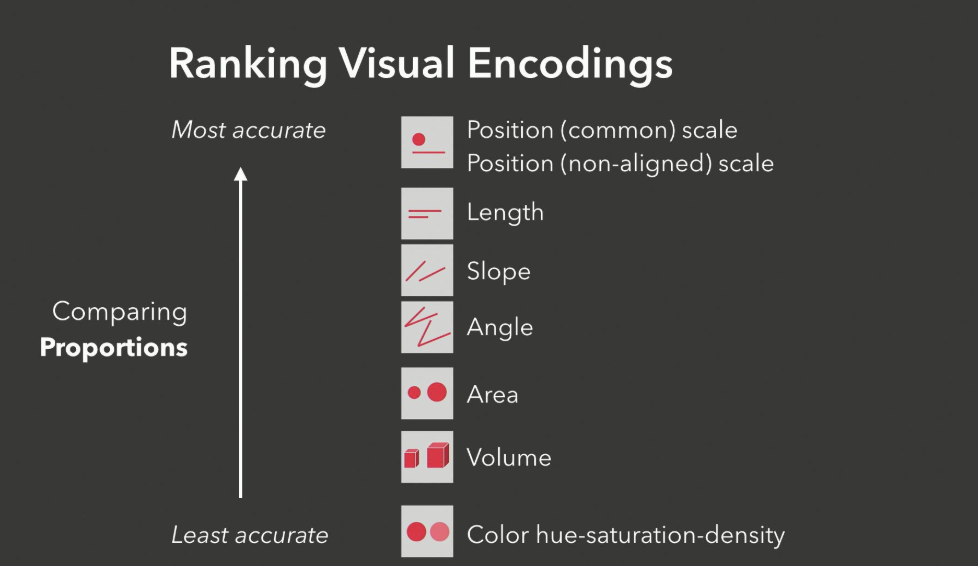
\includegraphics[width=0.7\textwidth]{figures/psychphys.png}
    \caption{Different accuracy for people in estimating quantities of visual stimuli}
    \label{fig:psychphys}
\end{figure}

{\bf Project:} Visual exploratory tool for large datasets, use inference in the background to automatically recommend new visuals. Can also be taught how to create these plots by the tool itself. \\

{\bf Key Idea from Demo:}
\begin{enumerate}
    \item Augment manual exploration with visualization recommendations sensitive to the user's current focus. 
    \item Ultimate goal is to support systematic consideration of the data without exacerbating false discovery.
    \item To model a user's search frontier, we optimize for related chart specifications, seeded current focus.
\end{enumerate} 
    

Representative quotes about the tool:
\begin{itemize}
\item Related view suggestion accelerates exploration a lot
\item I like that it show what fields to include to see a specific graph
\item The related views are so good but it's spoiling that I start thinking less. I'm not sure if that's a good thing
\end{itemize}

\subsubsection{Data Cleaning and Transformation}

Quote from Anonymous Data Scientist: {\it ``I spend more than half my time integrating, cleansing, and transforming data without doing any actual analysis. Most of the time I'm lucky if I get to do any 'analysis' at all"}

$\ra$ Responses; that can't be true! I wish I only spent 50\% of time on data cleaning.. (see big data borat on twitter).\\

{\bf New System:} DataWrangler (2011). DataWrangler: tool for generating relational datasets based on input preferences of user! Taught the system to automate aspects of the data cleaning process, but also generates a {\it program} that does the data cleaning. We can extract this program and use it for other thing, too.\\

$\ra$ ``Predictive Interaction": has an underlying domain specific language that can be used to ``lift" the program to generate visualizations and interactions. These lifted components can be used to inform a {\it guide-decide} loop for end users. \\

Also ran user studies with this system:
\begin{itemize}
\item Reduces spec time, promotes use of reusable scalable transformations.

\item Complementarity: suggestions good for tasks people found hard (extraction patterns, etc). People good in cases where inference is less tractable
\item Agency: Users appreciated suggestions in respond to an initiating interaction, but did not always act on practice assistance.
\end{itemize}

$\ra$ Company called Trifacta uses this interaction system and the discovered paradigms to scale the software to production. \\


\subsubsection{Natural Language Translation}

Started the talk with 1960s quote from Bar-Hillel---around this time there was a clear vision for interactive translation and interfaces. Even a proposal for an interactive translation workflow. \\



% \begin{figure}[h!]
%     \centering
%     \includegraphics[width=0.7\textwidth]
%     caption{Proposal for early interactive translation interface}
%     \label{fig:my_label}
% \end{figure}

$\ra$ Two big challenges, though: 1) Translation wasn't {\it good} enough to be a reliable collaborator, and 2) Getting these interface designs right is also challenges. \\

But! Revisited recently: predictive translation memory (PTM).

Again conducted user studies for interactive machine translation.
\begin{itemize}
\item Experiments with professional translators across language pairs (Arabic, French, German to English) and text genres (software, medical, news)
\item Results: 
\begin{itemize}
    \item Post-editing of full translation leads to reduced time and improved quality (over manual translation)
    \item Interactive translation with PTM slightly slower than post-editing but yields higher quality translations
    \item {\bf Similar concerns around agency:} ``I feel less susceptible to be creative", and ``distracts from my own original translation process by putting words in my head."
\end{itemize}


\end{itemize}


{\bf Design Challenge:} Determine regions of optimality in possible divisions of labor among directions and autonomous agents. \\

Future Challenges:
\begin{enumerate}
    \item {\it Design process, tools, and monitoring:} how might we support productive prototyping, development,  deployment, using machine learning?
    
    \item {\it Mapping machine-learned representations:} Can ML methods suggest structural task models? can people help test an constrain ML models?

    \item {\it Evaluating Trade-Offs of Agency and Automation:} Must go beyond results of quality and productivity.
    
    $\ra$ Locus of control, agency vs passive acceptance? Training and skill acquisition vs. de-skilled labor?
\end{enumerate} 




% ------------
% -- Friday --
% ------------
\newpage
\section{Friday December 13th: Workshops}
Today I will be at the Meta-Learning workshop!

\subsection{Workshop: Meta-Learning}

First up is an invited talk.

\subsubsection{Erin Grant on Meta-Learning as Hierarchical Modelling}

{\bf Main Idea:} Reformulate meta-learning as hierarchical modeling. \\

OpenAI released a chart that tracks the compute usage and identifies an inflection point in 2012 where compute went from a linear increase to an exponential increase. \\

$\ra$ Really different from the settings in which people solve problems. People can: 1) make sharp inferences given impoverished data, 2) adapt learning given computational constraints, 3) don't expereince lifetimes of data. \\

Lots of exciting questions here from both cognitive science perspective and machine learning. \\

Also: a major bridge between the two fields is {\it inductive bias}.
\begin{itemize}
    \item Shape Bias: in category learning, by the age of 2 years, English children exhibit the bias that shapes are generalized more rapidly than other properties like color.
    
    $\ra$ Cross linguistic differences attenuate the shape-bias.
    
    \item This is an example of a learned bias!
    
    Q: Can we formalize how such a bias could be acquired?
\end{itemize}

Yes! Work by \citet{kemp2007learning}. Model can reproduce shape bias on categorical learning task, both on known categories and novel categories.\\

$\ra$ Example of using ML tools to understand how biases arise in people. \\

{\bf Roadmap:}
\begin{enumerate}
    \item Main lcaim: recast meta-learning as hierarchical modeling
    \item Q: Why meta-learning as hierarchical modeling?
    \item Cast estimation/inference for parameters in hierarchical probabilistic models as a meta-learning framework for humans and machines
    \item Connecting these domains (cog sci and ML) can be mutually informative.
\end{enumerate}

{\bf Generic Recipe for Meta-Learning Algorithm:}
\begin{itemize}
    \item Sample a meta-train dataset:
    \[
    D_j \sim \mathscr{D}_{\tx{meta-train}}
    \]
    \item Learn task-specific parameters:
    \[
    \hat{\phi} \la g_\theta(D_j)
    \]
    \item Task-specific predictions:
    \[
    y_1, \ldots, y_n \la f_{\hat{\phi}}(D_j)
    \]
    \item Finally: do a global hyperparamater update to our main parameters
    \[
    \theta \la \theta - \nabla_\theta \mc{L}(f_{\hat{\phi}}(D_j)).
    \]
\end{itemize}

Q: Can we make this procedure probabilistic? \\

A: Yes! New recipe, same general formula:
\begin{itemize}
    \item Sample a meta-train dataset:
    \[
    D_j \sim \mathscr{D}_{\tx{meta-train}}
    \]
    \item {\it(Main Change)} Task-specific {\bf distribution}:
    \[
     p(\phi_j \mid D_j) \propto \int \prod_i p(y_i \mid \ldots )
    \]
    \item Then, updates involve updating:
    \begin{enumerate}
        \item Task specific predictive distribution
        \item Hyperprior update for general learning.
        \[
        p(\theta) \la p(\theta \mid D_i)
        \]
    \end{enumerate}
\end{itemize}

Problem! Probabilistic inference steps are now prohibitively expensive. Can we make this more efficient? \\

A: Yep: try hierarchical bayes. idea: don't maintain full uncertainty, use approximate empirical bayes to fit a point estimate via maximum likelihood:
\[
\argmax_{\theta} p(y_1, \ldots y_n \mid x_1, \ldots, x_j; \theta),
\]
rather than modeling the full posterior. Also need to do mode estimation. Trying to solve:
\[
\argmax_{\theta} p(y \mid X, \hat{\phi}) p(\hat{\phi} \mid \theta).
\]
Q: What is an appropriate way to represent the task parameters in a new domain? How do we formulate a local parameter prior?\\

A: Isotropic priors and early stopping might be able to help. \\

$\ra$ One approach that has this flavor is Model-Agnostic Meta Learning (MAML) \cite{finn2017model}. \\

Approximate Empirical Bayes: optimize marginal likelihood w.r.t. $\theta$ using a point estimate
\[
\argmax_\theta p(Y \mid X, \hat{phi}) p(\hat{\phi} \mid \theta),
\]
subject to:
\[
\hat{\phi} = \argmax_\phi p(y \mid X \phi) p(\phi \mid \theta).
\]
Similar to MAML:
\[
\argmin_\theta - L(X; \theta-\alpha\nabla_\theta L(X; \theta))
\]

But: gradient descent not the only way to compute a point estimate for these parameters. \\

Q: Can this estimate of $\hat{\phi}$ still be a valid point estimate for hierarchical Bayes?\\

A: Yes! When viewwed as an amortization of the MAP estimation
\[
\hat{\phi} = \argmax_\phi p(y \mid X) p(X \mid \phi)
\]

We can also go beyond point estimates; full empirical Bayes. Three approaches;
\begin{enumerate}
    \item Laplace approximation: LLAMA \cite{grant2018recasting}
    \item Sampling based estimate: Gibbs sampling, combinations of sampling techniques with variational inference
    \item Variational approximation: neural Statistication, Amortized Bayesian meta-learning.
\end{enumerate}

$\ra$ Another key way to make progress: is the underlying graphical model (from hierarchical Bayes) useful in the kinds of tasks we care about? \\

Apply these ideas to {\it continual learning} in which images are modified over time. Three phases: 1) image blur, 2) night mode, 3) pencil drawing filter. \\

Meta-test responsibility over time can identify when change points in the data occur. \\

$\ra$ Also investigate catastrophic forgetting as change point detection in this continual learning setting. \\

{\bf Conclusion:}
\begin{itemize}
    \item We can cast meta-learning as hierarchical Bayes, which allows a number of new insights.
    \item Can unify our understanding of meta-learning from hierarchical bayes
    \item Can draw inspiration from the probabilistic inference toolbox.
    \item Hopefully will bring closer links between human and machine learning.
\end{itemize}

Challenge Question: Bayes-optimal meta-learning is intractable, but is still exists. How do meta-learning produced by our current meta-learning algos compare to the Bayes optimal strategy, both quantitatively in terms of regret of qualitatively?\\

Erin Grant: Great question! Naturally these optimal forms are so intractable that we don't often focus on them too much. But I do think there is a big gap between optimal behavior and what we are achieving now. This is probably especially striking in RL, where exploration from a Bayes optimal perspective can help us view uncertainty in an optimal way. \\

\subsubsection{Jeff Clune on How Meta-Learning Could Help Us Accomplish our Grandest AI Ambitions}

Two main points today:
\begin{enumerate}
    \item Q: How might we produce capable AI?
    
    $\ra$ AI-generating algorithms!
    
    \item Exotic meta-learning approaches could help!
\end{enumerate}

Fruitful to think about the long term objective of the field. Yields some paths:
\begin{itemize}
    \item Manual Path to AI!
    
    $\ra$ Lots of building blocks: convolution, hierarchy, abstraction, (hundreds!)
    
    \item Once we identify these building blocks, we will need to combine building blocks into a giant Rube-Goldbergian complex thinking machine.
    
    $\ra$ Doesn't fit our scientific culture, doesn't lead to effective debugging and optimization.
    
    $\ra$ Might not even be possible.
    
    \item {\bf New Path:} Hand designed pipelines are ultimately outperformed by learned solutions: powerful path is {\it an all in bet on AI-generating algorithms.}
\end{itemize}

{\bf Main Idea:} Simple initial conditions that can be bootsrapped repeatedly to yield better and more capable algorithms. Darwinian evolution is one existence proof. Progress comes from three pillars:
\begin{enumerate}
    \item Meta learn architectures
    \item Meta learn algorithms
    \item Generate effective learning environments
\end{enumerate}

This talk is on work in these three pillars. \\

{\bf (Pillar 1):} Meta-learning architectures, as in architecture search.
\begin{itemize}
    \item Architectures matter
    \item Hard to design! So, let's search for them.
    \item Common approach: train on real data for moderate number of steps.
    
    $\ra$ Can be sped up by only doing a few steps of SGD, then use that to inform architecture design.
\end{itemize}

Lots of work that shows if we carefully select data we train on, we can speed data up a lot. \\

Q: Can we meta-learn to generate data that enables rapid learning?

A: Generative Teaching Networks---generates synthetic data, which a new network will train on for small number of steps. Then train new network on actual data, differentiate on the whole pipeline including the generator. \\

$\ra$ Empirical Finding: this works on MNIST and CIFAR10. Few-step accuracy is higher on synthetic GTN data than Real data. \\

GTN conclusion: can produce synthetic data that trains NNs faster than real data, enabling rapid estimates of an architectures performance. SOTA-competitve. \\

{\bf (Pillar 2):} Meta-learn algorithms. Two major camps;
\begin{enumerate}
    \item Meta-learn good weights and apply SGD: MAML ish
    \item Meta-learn rNN, which creates its own learning algorithm.
\end{enumerate}

Point: materials matter! Still have to decide the {\bf materials} of the network. RNNs forced to do all lifetime learning with activations: 1) may be unstable, and 2) proposal store information in weights too. \\

New work: Differentiable Hebbian Learning. Idea:
\begin{itemize}
    \item Can store info in weights in addition to activations.
    
    \item Train Hebbian learning via SGD
    
    \item Idea of Hebbian learning; ``neurons that fire together, wire together"
    \[
    w_{ij}^{t+1} = w_{ij}^t + \eta x-i^t x_j^t.
    \]
    \item Yields a recurrent Hebbian network.
    
    \begin{itemize}
        \item Inner loop: network update with no SGD
        \item Outer loop: differentiate through episode, update trainable parameters via SGD.
    \end{itemize}
\end{itemize}

$\ra$ Empirical finding: near SOTA on omniglot, also applied to maze navigation. \\

More work on Differentiable Neuromodulated Plasticity.
\begin{itemize}
    \item Hebbian learning is local: hard optimization problem!
    \item Better idea: turn learning on some weights, only in certain contexts.
    
    Example: If I am playing chess and I just wont, then I should increase learning in only chess playing parts of the network.
    
    \item Add a new filter to the Hebbian update to gate whether or not you update certain activations.
\end{itemize}

$\ra$ Empirical findings: performed similar experiments as in the Hebbian case. \\

New work: Learning to Continually Learn: specifically try to solve catastrophic forgetting.
\begin{itemize}
    \item catastrophic forgetting is the ``Achilles heel of machine learning"
    \item In sequential learning: cannibalize how to solve prior problems once new ones are introduced. We don't forget catastrophically.
    \item Must solve this problem to continually learn.
\end{itemize}

$\ra$ Many proposed approaches to solve this, but again we should use meta-learning. This work falls more into the MAML camp of meta-learning. \\

Meta-learning for continual, multi-task learning. \\

$\ra$ New work at NeurIPS this year: Online-aware Meta-Learning (OML) \cite{javed2019meta}. Idea:
\begin{itemize}
    \item Meta-learns a representation network
    \item At inference time, freeze this representation network, and a new task learning network will learn on top of the representation.
    \item Gets a lot right!
    
    $\ra$ Subject to the ``tyranny" of SGD during learning: not optimized for continual learning.
\end{itemize}

New Proposal: allow for control over SGD via neuromodulation. This yields; A Neuromodulated Meta-Learning algorithm or ``ANML". Two networks; 1) Neuromodulated network, and 2) Task network. \\

$\ra$ Empirical work on sequential variation of Omniglot, following OML. \\

ANML conclusions: OML and ANML show the promise of meta-learning a solution to catastrophic forgetting. \\

{\bf (Pillar 3):} Generating the right environments. \\

Q: How do we get the right tasks? \\

Another variant: Can algorithms generate their own problems while learning to solve them? \\

$\ra$ Inspired by open-ended algorithms that endlessly innovate. Examples: 1) Natural evolution, and 2) Human culture. Both of these generate their own problems while they're trying to solve them. \\

New approach: POET. Periodically generates new learning environments that are in the ``Goldilocks" zone (not too hard, not too easy). \\

$\ra$ Deploy in RL, generates environments and tries to solve them. Empirical finding: learns well on these problems, but also learns to find a better solution on the simple tasks after seeing the harder tasks. \\

POET conclusions: invents effective curricula, endlessly innovates, captures spirit of open-ended innovation engines, fuels meta-learning \\

{\bf Overall Conclusions:}
\begin{itemize}
    \item Let's take a step back: is the manual path to powerful AI the fastest?
    \item AI-Generating algorithms is an all in bet on meta-learning
    \item Three pillars: 1) meta-learn architectures, 2) meta-learn learning algos, 3) generate algorithms.
\end{itemize}

Challenge Question: When does neuroevolution outperform?\\

Jeff Clune: Naturally thee optimization algorithm is going to make a big difference. We often confuse evolution the optimization algorithm vs. algorithms inspired by evolution (such as POET). Final answer: if we do actually compare evolution to other optimizers, it doesn't require gradients, more stable, and leads to different behavior; different exploration profile, can escape local optima, care about population rather than individuals. \\

\subsubsection{Spotlight: Meta-Learning Contextual Bandit Exploration}

Talk by Arvin. \\

Q: Can we learn to explore in contextual bandits? \\

A: Yes! Meta-learning.

\ddef{Contextual Bandit}{Interactive learning setting constituting a bandit problem where each step comes with a context feature that describes something relevant about the current bandit.}

$\ra$ Allows for study of generalization and exploration. \\

Solution: At meta-training time, assume access to $\pi^*$ that knows how to explore/exploit and use it to train. \\

Q: What happens when we don't have access to $\pi^*$? \\

A: Generalization via meta-features!  \\

$\ra$ Compare approach in a variety of contextual bandit problems, find significant improvements in most settings. \\

Theoretical guarantees: no regret property of ``Aggrevate" can be leveraged here too.


\subsubsection{Spotlight: ES-MAML: Hessian Free Meta Learning}

Talk by Wenbo Gao. \\

Objective: applying {\it evolutionary strategies} (ES) to MAML. \\

Key Q: Can we perform meta-learning in blackbox case? \\

A: Yes! Through ES methods which perform gradients on Gaussian smoothing of function. \\

Toy problem: four corner task. Agent gets reward signal if close to the corner of a continuous grid. \\

$\ra$ ES-MAML adaptation targets only 1 or 2 corners while policy gradient (PG) MAML must ``circle around" all 4 corners. \\

$\ra$ Further compare ES-MAML vs. PG-MAML, find: 1) ES-MAML is more stable, and 2) allows the use of non-smooth adaptation methods, yields new algorithmic design choices.


\subsubsection{Spotlight: Quantile Based Approach for Hyperparameter Transfer Learning}

Setting: assume many possible hyperparameter (HP) evaluations, want to find the best for transfer. \\

$\ra$ Difficulties, though: 1) sacles of objectives may vary across tasks, 2) noise may not be Gaussian, and 3) many observations so it's hard to apply approximate Gaussian Processes. \\

New idea: Gaussian Copula transform:
\begin{itemize}
    \item If only every $y'$ was Gaussian, we could use GPs!
    \item So: apply change of variable $\psi = \phi^{-1} \circ F$
    \item Can prove this transform yields a centered normal distribution.
\end{itemize}

Idea: do transfer learning by estimating a transfer variable, then learn the parameters of a Gaussian distribution. \\

Two new hyperaparameter optimization strategies: 1) Thompson sampling, and 2) Gaussian Sampling. \\

$\ra$ Evaluated on several dataset and find large improvements to learning.

\subsubsection{Spotlight: Meta-World: Benchmark for Meta-RL}

Previously: in multi-task RL, use things like DMLab and Atari games for testing. \\

$\ra$ However: tasks are relatively disjoint. \\

$\ra$ In Meta-RL, mostly use tasks that are very similar to each other. \\

{\bf Goal:} To enable the generalization ability of Meta-RL algorithms. We need a large diverse task set, which is what Meta-World is.
\begin{itemize}
    \item 50 qualitatively different manipulation tasks using a simulated sawyer robot
    \item Parameter variability
    \item Unified observation and action space
    \item Structured, multi-component rewards for all tasks.
    \item Also include benchmark results for meta-RL algorithms.
\end{itemize}

Videos and code: \durl{http://meta-world.github.io/}

\subsubsection{Pieter Abbeel: Better Model-based RL through Meta-RL}

{\bf Talk:} Share work on how meta RL can help model based RL (MBRL). At the end: show how we can make meta-training more efficient.\\

Overview:
\begin{enumerate}
    \item Learning to RL
    \item Domain randomization
    \item Better MBRL through Meta RL
    \item Speeding up Meta RL training
\end{enumerate}

{\bf Part I:} Learning to RL \\

Q: How fast can we learn? \\

A: People can learn a game in around 15 minutes, while DDQN takes 1500 hours! \\

Main Q: How can we bridge this gap? \\

Ideas:
\begin{itemize}
    \item Humans might play Atari for first time, but have done lots of similar things before.
    \item So, let's let RL systems learn on previous tasks, then generalize its knowledge to the new tasks.
\end{itemize}

Formulation: end-to-end optimization problem. Searching for an RL agent that can, on expectation, learn quickly:
\[
\max_\theta \bE_m \bE_{\tau_M}\left[\sum_{k=1}^K R(\tau_m^k) \mid \tx{RLAgent}_\theta\right].
\]
The setting is then about finding these agents via meta-training. Generate training environments that enables agents to learn to do well on the test environment. \\

Q: How do we represent $\tx{RLAgent}_\theta$? \\

A: RNN! Since it's a generic computation architecture, it can learn programs/algorithms. Different weights in the RNN means different RL algorithm and prior. Different activations in the RNN means different current policy. \\

$\ra$ Objective: it's the same as a usual RL algorithm but instead of a new state, we get dropped into a new environment. So, pick your favorite RL algorithm to optimize the meta-objective. \\

Evaluation:
\begin{enumerate}
    \item Multi-Armed Bandits: simple, focus only on exploration.
    
    $\ra$ Can then compare what a meta-RL agent does compared to the asymptotically optimal (Gittins) approach.
    
    \item Navigation in Mazes: agent gets first person view of a 3d environment, looking for a treasure in a maze.
    
    $\ra$ Random exploration fails, but after meta-training, meta-RL agent learns an algorithm for systematically exploring the maze to find the treasure.
\end{enumerate}

{\bf Part II:} Domain Randomization. \\

Q: Why do we care about simulation? \\

A: Less dangerous, easy to get labels, faster/more scalable. \\

$\ra$ But! Of course it doesn't match the real world. \\

Follow up Q: how can we learn useful real world skills in simulation? \\

A: That's what domain randomization is for. \\

$\ra$ If the model sees enough simulated variation, the real world may look like just the next simulator. \\

Initial results: quad copter flight can train in simulation with domain randomization $\implies$ copter learns to fly in the real wworld. \\

$\ra$ Q: Can we just train on unrealistic simulators like ImageNet, but randomize a lot? \\

A: Yes, actually! Evaluate on real world data and the approach works quite well. Used for robotic grasping, too. Real world is able to pick up objects in the real world based on simulated training alone. \\

{\bf Hypothesis:} Training on a diverse array of precedurally generated objects can produce comparable performance to training on realistic object meshes. \\

$\ra$ Even harder challenge: in hand robotic manipulation.
\begin{itemize}
    \item By training on wider range of randomized simulators, can learn to manipulate a block
    
    $\ra$ Super challenging because contact forces are highly complicated.
    
    \item Goal is to orient a cube with letters on it to a particular angle.
    
    \item Robot learns to do manipulate these blocks from simulation alone, also extension to rubix cube.
\end{itemize}

{\bf Part III:} Better MBRL through Meta RL \\

\ddef{Model-Based RL}{Model-Based RL uses experience to learn a simulator that we can use to train our behavior.}

Canonical MBRL:
\begin{enumerate}
    \item Colllect data under current policy
    \item Improve learned simulator from all past data
    \item Improve policy in learned simulator.
\end{enumerate}

Problem! Standard overfitting in ML rears its head.
\begin{itemize}
    \item Policy optimization tends to exploit regions where insufficient data is availablle ot train the model, leading to catastrophic failures.
    
    \item Model-bias: see \citet{atkeson1997comparison}, or \citet{deisenroth2011pilco}.
    \item Idea: Just learn a better model?
    
    $\ra$ Use the two tools we discussed: 1) Domain randomization, and 2) Meta policy optimization.
\end{itemize}

Canonical MBRL with Meta Policy Optimization (MB-MPO):
\begin{enumerate}
    \item Collect data under current adaptive policies $\pi{\theta_1}, \ldots, \pi_{\theta_n}$.
    \item Learn ensemble of K simulators from all past data
    \item Meta-policy optimization over ensemble:
    \begin{enumerate}
        \item New meta-policy $\pi_\theta$
        \item Net adaptive policies $\pi{\theta_1}, \ldots, \pi_{\theta_n}$.
    \end{enumerate}
\end{enumerate}

Experiemnts in Cheetah: MB-MPO compared to PPO. Learns in a much more sample efficient way. Achieves state of the art relative to model-free approaches in Mujoco 9Ant, HalfCheetah, Hopper, PR2, swimmer, Walker2D). \\

$\ra$ Compare wall-clock time as well of robotic grasing/lego block stacking $\ra$ achieves very quick learning even relative to wall-clock by training {\bf asynchronously} (on the order of 10 minutes). \\

{\bf Part IV:} Speeding up Meta RL Training. \\

We do meta RL in part because we want to get away from the sample complexity of RL. \\

$\ra$ But! Meta training can be just as demanding in terms of sample complexity. \\

All we want is a fast RL algorithm. We can make the meta training faster by matching the outer policy to a policy we trained on that task already: now it's a supervised loss rather than RL. Requires a policy on a few specific tasks, but can be a lot more efficient than doing full meta RL. \\

Experiments in pushing and opening doors and locomotion tasks. \\

Challenge Question: Recently seems to be a push in MBRL. Techniques from representation learning seem promising to learn helpful representations for more efficient planning. Any intuition on how to choose suitable objectives for learning good representations for MBRL? \\

Pieter Abbeel: Learning better representations is a really important research direction. It's probably large under researched to find better architectures for Meta-RL. In principle, in meta learning memory should play a big role. Smarter architectures could play a big role in improving these results. In MBRL, if we think about where model learning could make a big difference, it's really about reasoning over long horizon. Lots of benchmarks that are sample efficient with MBRL are still short horizon. Big question: how can we get simulators that simulate over long horizons in a reliable way.


\subsubsection{Panel Discussion: Erin Grant, Jeff Clune, Pieter Abbeel}

{\it Q: How should we design Meta-learning training task distributions?} \\

PA: Big challenge in meta-learning! Recent work on MetaWorld contains 50 robotic maniuplation tasks. Good solution. Still seems to be on the lower side. Most important direction is to, in some unsupervised way, generate the right tasks. Use some very objective but light weight principle to generate the task distribution. \\

JC: Unsurprisingly I'll agree with Pieter. We ultimately want to automatically generate the tasks. Continue to fan out tasks. Unknown unknown problem: might be things we don't think about to include. For that, I advocate for the POET style that automatically generates environments. Allow the search algorithm to choose which worlds to learn from. Opens the floodgates to learning a wide distribution of tasks. \\

EG: Can be turtles all the way down. Some way we have to provide inductive bias to our learning algorithm. What meta-learning does it remove constraints from the learning algorithm to instead apply constraints to the data set. Nevertheless we do have to specify some manner of bias to generate datasets. Needs to be a balance between things the agent can reasonably solve and things it can't. Perhaps instead of thinking about functional priors instead of smoothness/locality, we should be thinking about the kinds of invariances we might an agent to pick up on. \\

JC: Another thing---what is the curriculum that's going to get you to solve some harder task? The whole curriculum can't be full of hard tasks. One way to solve that is a distribution that winds you up in complexity. Learn the tasks that help you learn. \\

PA: Want to add one thing to Erin's point. Might not be that easy to generate or design environments. Before humans were ruling Earth, dinosaurs were around. They were in some sense in a very similar environment to us. But, there was something different that led to intelligence. \\

EG: Could we speculate about what it is about the environment that changed that enabled humans to be intelligent? \\

PA: Not sure! Maybe the dinosaurs developed their bodies rather than their brains. \\

{\bf Q: Is there a limit to how much we can learn via Meta RL? Will we hit no free lunch?} \\

EG: Reasonable hypothesis that the world has structure. Wouldn't want to be a nihilist in that sense. Maybe it's too complex to characterize in a learning system, but there is some structure that can be picked up on so agents can learn to quickly solve a variety of tasks. \\

JC: No free lunch doesn't keep me up at night because the space of problems is so vast. We don't care about algorithms that get better at these white-noise TV problems. We can focus our algorithms on ones that are relevant to our world. What does keep me up at night is generating tasks that are grounded in the real world in the relevant sense. \\



\dnote{Need to run to lunch so missing the rest of the panel. Also, my talk is up next! So, no notes.}

\subsubsection{Raia Hadsell on Scalable Meta-Learning}

Note: Learning from i.i.d. data is strange! Think about how we learn? Think about how we learn philosophy, Latin, biology, and so on: we don't randomly sample lessons/textbooks and learn. There's a curriculum! \\

$\implies$ We learn best by prolonged inspection and consideration of one subject at a time. \\

Q: How fast should learning be? How quickly should a learning algorithm adapt? \\

A: Transfer and generalization are central problems in machine learning. Deep learning approaches refuse to cooperate on these problems. \\

Q: How slow should learning be?
A: Learning to optimize behaviour from extensive experience in an environment. Evolutionary optimization, for example. Slow and potentially not robust nut highly optimized. \\

Need: slow learning {\it and} fast learning! \\

Alternate title of this talk: learning as a not-too fast, not--to slow, non-stationary, non-i.i.d. process! \\

Exploring the potential for scalable meta-learning methods: Learning from memory, learning to compare, and so on. \\

Paper: Meta-learning with warped gradient descent \cite{flennerhag2019meta}.
\begin{itemize}
    \item Main insight: Learning  a geometry does not depend on the initialization -- only on the search space!
    \item In WarpGrad, learn to precondition gradients over a search space.
    \item SGD defines an empirical parameter distribution of this process.
    \item A new efficient few-shot learner, but can also handle complex architectures and problems.
    \begin{itemize}
        \item Maze navigation task vs. A2C RNN agent.
        \item Hypernetwork as warp-layers
        \item Trained online with periodic meta updates.
        \item Also experiments on continual learning.
        
        $\ra$ Main result: network learns to both parition and share capacity.
    \end{itemize}
\end{itemize}

Next up: Learning from Memory, from upcoming paper ``Stabilizing Transformers for RL"
\begin{itemize}
    \item Transformers are extremely powerful memory architectures: also no vanishing/exploding gradients, arbitrary indexing over time, receptive fields only limited by accelerator memory.
    
    \item Recent breakthroughs surpass recurrent models by large margins!

    \item But, vanilla transformers are hard to optimize! Lots of attempts at using transformers:
    \begin{itemize}
        \item DMLab30: attempts at memory unsuccessful.
        \item Unstable
        \item Did not even match basic performance
    \end{itemize}
    \item Further reported difficulties: ``Hypothesize transformers inadequacy stems from the fact that pure attentive lookups cannot easily process sequential information.
    
    \item New algorithm/architecture: GTrXL, uses transformers and gating variations in RL.
\end{itemize}

Results:
\begin{itemize}
    \item On DMLab 30: 3d, first person view POMDP problems that often require memory to solve puzzles. Lots of variations in tasks.
    
    \item Achieves SOTA on this set of tasks, comparing to MERLIN (Memory, RL, and Inference Network) \cite{wayne2018unsupervised}. Lots of complexity in MERLIN: memory-based predictor, read-only policy, huge number of losses/coders/decoders.
    
    \item In contrast: new transformer based approach (GTrXL) is quite simple, but still achieves roughly the value of MERLIN.
\end{itemize}

High level: 1) started with transformer (TrXL), then 2) moved to TrXL-I (adds a layer norm, moved inside the residual connection), then 3) added a gating connection between the residual and output of the previous layer (GTrXL). \\

$\ra$ Tried several kinds of gating variants, from Highway, PixelCNN, to a GRU-type, found that GRU worked the best. Extension ablation studies to understand each component (compare \# parameters with mean human normalized score on DMLab30). \\

Numpad task: a continuous control memory problem.
\begin{itemize}
    \item A 3d represented set of buttons on a pad; $N\times N$ grid of buttons. Agent has to move a cursor over the pad in the right pattern.
    \item Continuous action space
    \item State observation space
    \item 500 episodes.
    \item New memory-based approach can work quite well on these hard memory control problems!
\end{itemize}

Q: How does this relate to Meta-RL?
\begin{itemize}
    \item A recurrent network can encode the dynamics of current environment and adapt policy without further parameter optimization.
    \item A transformer learning to use attention over the experience buffer.
\end{itemize}

\dnote{I missed the challenge Q :(}


\subsubsection{Spotlight: Meta-Learning with Warped Gradient Descent}

Background: meta-learning is all about transfer across learning {\it processes}, rather than structures. \\

$\ra$ Depending on what the learning process is, we get different meta-learning types. \\

MAML \cite{finn2017model}: learn an initialization for good final performance. Learning as a function:
\[
\mc{F}(\theta_0) = L(\theta - \alpha \nabla L(\theta)).
\]

Powerful idea! But, hard to scale: 1) Vanishing/exploding meta-gradients, 2) Computationally costly, 3) Hard to make wwork for more than 10 adaptation steps. \\

{\bf Main Question:} Can we come up with a gradient-based meta-learner that is not a function of the initialization? \\

$\ra$ Key insight to get it to work: rather than taking the loss surfaces as a given, {\it warp} it by learning a projection $\gamma = \Omega(\theta;\phi)$. \\

$\ra$ This is equivalent to learning a gradient ``preconditioner": $P(\theta) \nabla \mc{L}(\theta)$. \\

Meta-learning now means:
\begin{enumerate}
    \item In WarpGrad, learn precondition gradients ove search space
    \item SGD defines empirical parameter distribution over this space
    \item Meta learn warp parameters to yield steepest descent.
\end{enumerate}

Experimental findings:
\begin{itemize}
    \item Few-shot adaptation: works quite well!
    \item Also goes beyond trivial few-shot adaptation to methods that MAML based methods didn't work on.
    \item Extend to RL on maze navigation tasks based on an A2C rNN agent.
\end{itemize}

Conclusion:
\begin{itemize}
    \item WarpGrad is an effective and scalable gradient-based meta-learner
    \item WarpGrad is a flexible parameterization of an optimizer
    \item Next steps: what are the effective architectures for warp layers?
\end{itemize}

\subsubsection{Spotlight: Meta-Pix: Few Shot Video Targeting}

Talk by Jessica Lee. \\

Problem: video retargeting. Goal is to translate information from a source video to a new video. \\

$\ra$ Pior work: ``everybody dance now" \dnote{I've seen this, it is mind blowing! Check out the videos}. \\

Problem with prior work, though: requires a massive dataset of prior dance. \\

{\bf Goal:} Generate a video of a person given a few samples of their appearance. \\

Two approaches under ``pose-guided image synthesis":
\begin{enumerate}
    \item Pose2Im: methods learn a model specific to a person and background (sort of like model-based RL, it seems).
    
    $\ra$ Same problem as everybody dance now: data hungry.
    
    \item Pose Transfer: transforms a source image directly into a target image.
    
    $\ra$ Prior work: ``Dance Dance Generation"
\end{enumerate}

Q: Can we reduce this data requirement? \\

Approach: MetaPis---learn a general model that can be efficiently and quickly adapted to an appearance via meta-learning. Combine REPTILE (first order method) and Pix2VAE. \\

Pretraining dataset: 10 dance videos from youtube. Follow roughly the same evaluation protocol as the Dance Dance Generation work. \\

Baselines: random weights, pretrained weights, and MetaPix. \\

Qualitative results: videos of people being puppeteered in videos, seems to work quite well! \\

Also include quantitative evaluation and ablation studies (including some very cool visuals of pretraining and fine tuning process). \\

Conclusions:
\begin{itemize}
    \item Meta-learning as a personalization technique.
    \item Meta-training as a generative model provides insights to what meta-learning captures
    \item Image synthesis as a meta-learning task.
\end{itemize}

Code: \durl{github.com/imjal/metapix}

\subsubsection{Brenden Lake on Compositional Generalization in Minds and Machines}

{\bf Goal:} understand {\it systematic compositionality}: the alhebaric capacity to understand and produce novel combiations from known components. \\

Example: ``This is how you dax" (swirl your hand above your head). Now dax twice! Backwards! while jumping! We can do this. \\

Central Qs:
\begin{enumerate}
    \item Do modern AI models show systematic compositionality?
    \item How do people make compositional generalizations
    \item Can compositional skills be acquired via meta learning?
\end{enumerate}

Q: Do neural language models show systematic compositionality? \\

$\ra$ Sequence task to train a model to follow commands. Ex: Walk, then jump after walk, move to the left, and so on. Given this sequence of commands, needs to parse these commands into a predicate like language. \\

Zero-shot evaluation: never seen this precise command. \\

SCAN learning setup:
\begin{itemize}
    \item 21k commands and corresponding action sequences
    \item Simplifications: no scope ambiguity, no recursion
    \item Evaluate Seq2Seq RNNs on SCAN with an extensive hyperparameter search.
\end{itemize}

SCAN Experiments
\begin{enumerate}
    \item First, use a random train/test split, where test always consists of new and composed commands.

$\ra$ Neural net masters zero-shot generalization with about 8\% coverage in training (1,650 of 21,000 commands).

\item Generalizing to longer action sequences.

    $\ra$ Neural net fails to generalize to novel longer sequences, even though all sub-commands are familiar.

\item Composing a new primitive (like the ``dax" experiment): all primitives except one are used in training, new primitive ``jump" only seen in a few contexts.

$\ra$ Neural net has difficulty incorporating new primitive and shows patchy generalization (fails on all conjuncts of ``dax thrice" or ``dax", while ironically succeeding on ``dax thrice and dax").
\end{enumerate}

Insights from SCAN: 1) Powerful Seq2Seq models can do zero-shot generalization to novel compositional instruction, but still far from systematic generalization, and 20 Current models are missing the ability to abstract systematic rules and variables (Marcus, Pinker, etc). \\

Ex: ``Do $X$ and $Y$" should be learned as a rule with {\it variables}, where we can seamlessly plug in new $X$ and $Y$. \\

Back to people: how do people solve this? Why are people better compositional learners than neural nets? \\

$\ra$ Let's collect some data about how people learn patterns.
\begin{itemize}
    \item Built a dataset where people are given instructions (pseudowords like ``dax" and ``zap") with responses (abstract like red circle).
    \item Four primitives, based around compositionality.
    
    $\ra$ No scope ambiguity.
    
    \item As suggested above, most neural nets fail miserably on all of the tasks.
\end{itemize}

Behavioral experiment 1: Design. Told participants to ``learn a set of commands and their corresponding outputs". Outputs produced by dragging symbols from a pool of options. \\

Results ($n=20-25$):
\begin{itemize}
    \item Overall performance when applying to a {\it novel input variable} was $\approx 85\%$.
    
    \item Achieved 76\% accuracy when composing function in new ways
\end{itemize}

\begin{figure}[h!]
    \centering
    \subfloat[Examples]{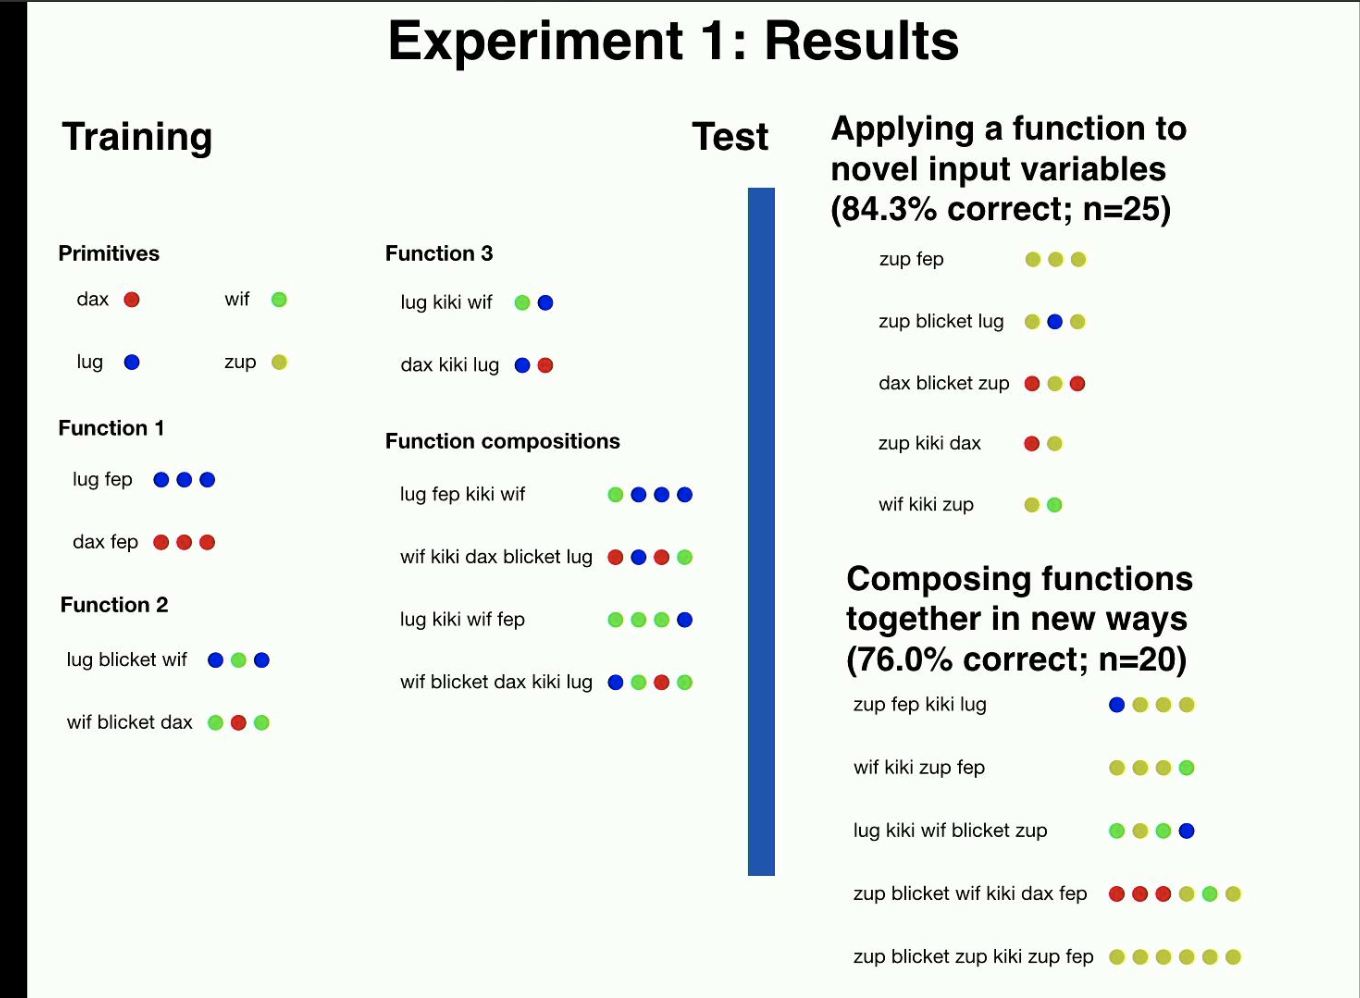
\includegraphics[width=0.42\textwidth]{figures/dax_blicket.png}}
    \subfloat[Inductive Biases]{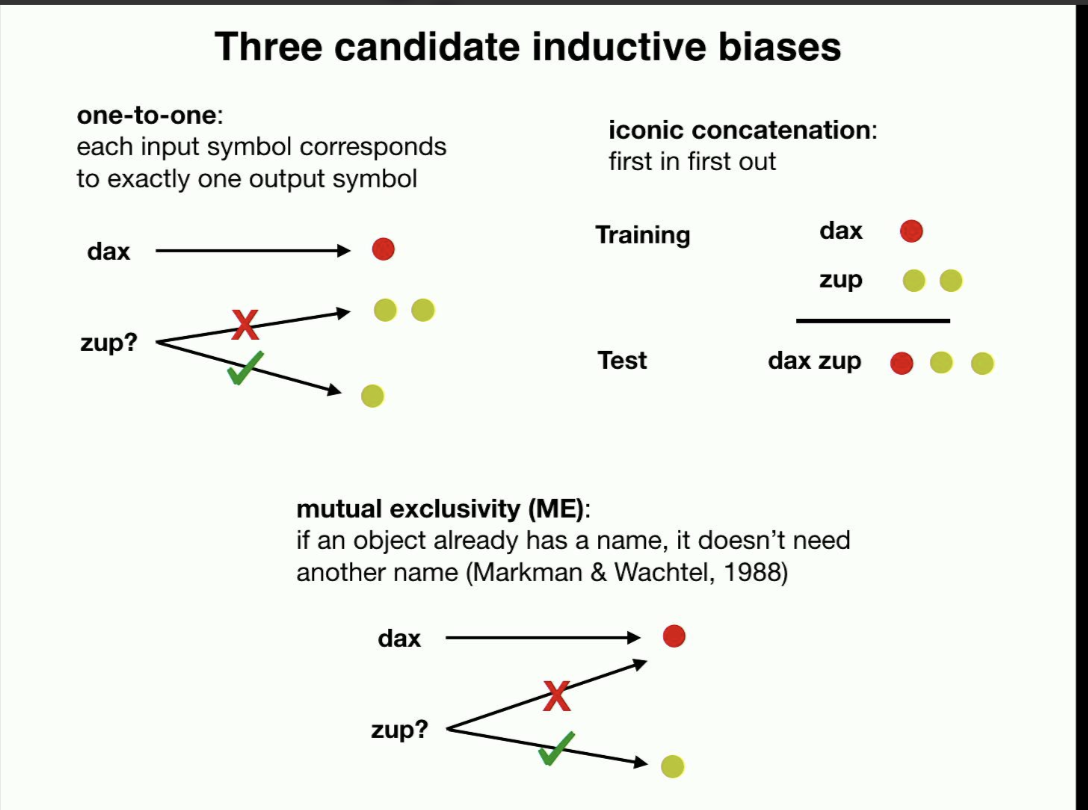
\includegraphics[width=0.42\textwidth]{figures/ind_bias.png}}
    \caption{Some examples from the dataset (left) and visuals of inductive biases (right).}
    \label{fig:blicket}
\end{figure}

Summary: find several inductive biases in participants such as $\ra$ 1) one-to-one: people like these mappings, 2) iconic concatenation(first in first out), and 3) mutual exclusivity: everything has {\it one} name, not more. \\

Experiment 2: free-form prompts, examine inductive biases on seq2seq task with NO training examples. \\

$\ra$ More than a source of error, these biases provide critical inductive constraints. \\

Central Q: Can compositional skills be acquired through meta-learning? \\

Goals:
\begin{itemize}
    \item Want a structured neural network that can:
    \begin{itemize}
        \item Learn new primitives and use the compositionality
        \item Encode inductive biases
        \item Capture rich starting point people bring to compositional learning tasks
    \end{itemize}
    \item Do NOT intend models to explain developmental process, resolve which components are learned vs. innate.
\end{itemize}

New work that tries to capture the above goals: Meta sequence-to-sequence learning \cite{lake2019compositional}.
\begin{itemize}
    \item Learning is distributed over a series of dynamically changing datasets that encourage compositional generalization
    \item Training episodes contain thousands of support/query set.
    \item No weight updates at test set.
    
    \item Architecture has RNN encoders for the support, passed with attention to a decoder.
    
    $\ra$ But, meaning of words is changing between episodes! So can't learn a fixed mapping.
\end{itemize}

Q: Can a network acquire human-like biases? \\

A: Yes, it seems! Results: achieved 100\% on quickly acquiring new mappings. \\

$\ra$ Also applied to SCAN: evaluated on new episodes with original mappings. Meta seq2seq achieves 99.95\% on adding ``jump" (the piece that broke earlier models). \\

Coming back to ``dax": both people and the model can learn a new verb and use it compositionally. Model needs to see a lot of combinations of similar pairs, though. \\

{\bf A Step Back:}
\begin{enumerate}
    \item Wanted a framework that can:
\begin{itemize}
\item Learn new primitives and use the compositionality
        \item Encode inductive biases
        \item Capture rich starting point people bring to compositional learning tasks
\end{itemize}
\item We now have those three properties!
\item Lots to do though: 1) modeling details of human behavior, 2) acquire human priors, 3) Learn new primitives, 4) Understand how these abilities develop, 5) Large scale compositional word learning.
\end{enumerate}

Started with the question: ``what are the computational underpinning of human compositional skills?" Studied:
\begin{enumerate}
    \item Powerful seq2seq models fail spectacularly when systematic compositional skills are required
    \item People can learn new concepts and apply them in new ways
    \item Structured, memory-augmented networks can perform few shot composition.
\end{enumerate}

Challenge Question: How do we know what the right inductive biases are? \\

Brenden Lake: We should look to cognitive development! Early emerging abilities are likely to be most important. We should study computational problems that are easier fr people than for machines. Collect behavioral data and reverse engineer human inductive biasers. I see meta learning as a tool for encoding priors in cognitive modeling or machin learning that are too difficult to specify by hand or easier to specify in data than an explicit prior. In the Bayesian sense, we want a put a prior on our model but it's hard to specify: meta-learning can be an effective way to specify complex priors. \\

\dnote{And that's a wrap! I'm doing the panel now.}




% ------------
% -- Saturday --
% ------------
\newpage
\section{Saturday December 14th: Workshops}
I had meetings the whole day! I caught a few minutes of the OptRL panel

\subsection{Panel at OptRL: Doina and Rich}

{\it Q: Are you happy with the balance of engineering vs. theory in RL?} \\

Doina: From my point of view we are trying to do good science and want to be building algorithms that we understand. What does it mean to understand algorithms? In the past this has often meant theory: convergence, PAC bounds, etc. But in some cases the theory can't yield understanding: vacuous bounds, hard to analyze cases, mismatch from real world, and so on. So, what we need is a concerted effort to make theory {\it meaningful}, and to make our experimental analysis more thorough in the sense of trying to understand what is going on, even in large scale experiments. Not necessarily theory but might point out new directions for theory. \\

Rich: Well, Doina, that's a very bold point of view you have that it's all about science! I have a hard time disagreeing. The engineering and experimental pieces are also really important. Every field has to deal with this clash. There shouldn't be a conflict. Any field, engineering or science, shoudl be like a conveyor belt: at one end you put in big ideas and practice, and at the other end you output a better deeper theoretical understanding. There is a natural drift toward experimental work. The goal is to increase understanding. You have to start with things you don't understand! We need new things on the conveyor belt so we understand more over time. \\

Doina: From a theoretical point of view, people say RL is very hard; but, that makes it very exciting! It's a good time to do theory in RL. After stalling for some number of years now we have momentum. \\

Rich: I totally agree. The field is hard because we're working with fundamental questions. I think about it as how intelligence works, how to achieve goals, and so on. The more we get to the core of these key problems, we should expect them to be challenging. Don't be discouraged when you do hard things! The real conclusion is that we have to value incremental progress on hard problems. A small amount of fundamental progress is a big deal. \\

\dnote{Had to run to meetings :(}



\subsection{Talk at Deep RL: Michael Littman on Assessing the Robustness of Deep RL Algorithms}

Background:
\begin{itemize}
    \item Started off interested in explainable RL: why does DQN choose the moves it does in Atari?
    
    \item Ended up wondering if any explanation at all is possible
    \item {\bf Punchline:} Generalizing Q values is hard!\cite{witty2018measuring}
\end{itemize}

Case study 1: Amidar! DQN can do extremely well on this game. \\

$\ra$ But: can we look at one of the moves and figure out {\it why} it made this decision? \\

To answer this:
\begin{itemize}
    \item An explanation is something that tells us how things would have been if something else happened.
    \item Tried causal interventions:
    \begin{enumerate}
        \item Idea one: Prefill one of the boxes! Think Pac-Man with some random pellets missing (couldn't have reached the state).
        
        $\ra$ Agent stops moving entirely and starts to be killed.
        
        \item Next up: get rid of the enemies! Same game (again think Pac man with no ghosts).
    \end{enumerate}
\end{itemize}

$\implies$ Takeaway here: DQN doesn't {\it really} know how to play the game! All it does is learn a good strategy, but it's very brittle. \\

Next up: investigate {\it saliency}. Ask: what makes big changes in action choice or value prediction if blurred out? What does the learned netwwork pay attention to? \\

$\ra$ Memorized movement! \\

So: maybe we're thinking about learning wrong. Let's go back to {\bf supervised learning}. How do we measure success?
\begin{itemize}
    \item how well it does on training set
    \item Interpolation: How well it does on test/validation set(s)
    \item Extrapolation: How well it does on out of distribution data
\end{itemize}

Analogues in RL, though:
\begin{itemize}
    \item Training examples $\ra$ On policy states
    \item Interpolation $\ra$ Off-policy states
    \item Exrapolation $\ra$ unreachable states.
\end{itemize}

Q: How can we test these different kinds of generalization/states in RL? \\

A: Different interventions! Off-policy: push to different states, force to unreachable states, and so on. \\

Evaluation Metrics: 1) Value Estimation Error (VEE): how far off is Q error?, and 2) Total Accumulated Reward (TAR). \\

\begin{figure}[h!]
    \centering
    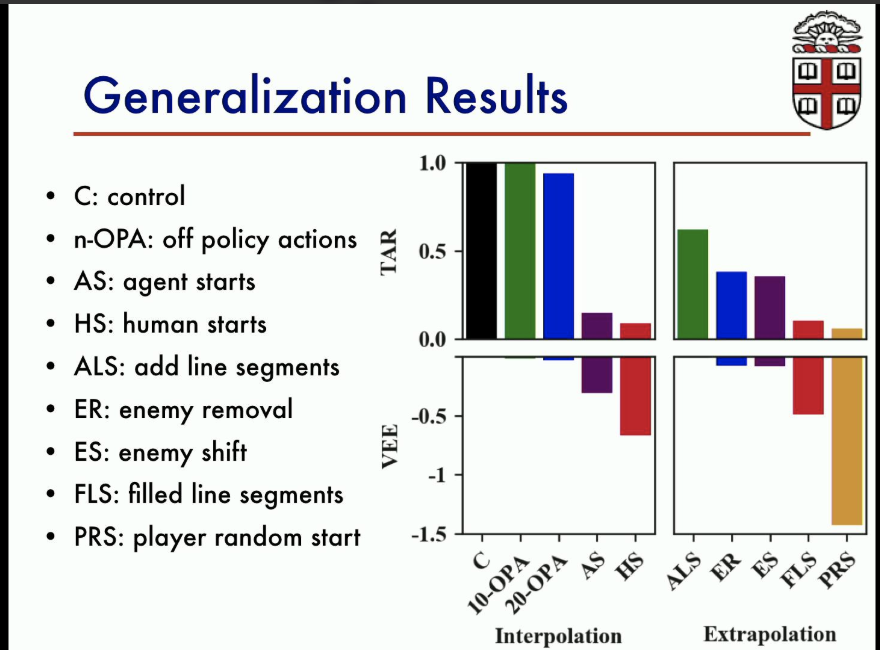
\includegraphics[width=0.7\textwidth]{figures/gen.png}
    \caption{Results on generalization types for RL}
    \label{fig:gen}
\end{figure}

Findings:
\begin{enumerate}
    \item Full results in Figure ~\ref{fig:gen}.
    \item VEE and TAR correlate.
    \item Novel states not recognized! Learned representation does not find the novel states to be similar to those seen in training (via activation analysis).
\end{enumerate}


Q: So how can we improve generalization? \\

A: Well, in supervised learning, we do a few things: 1) more data, and 2) less model (regularization). \\

Q: So how about in RL? \\

A: A few things: 1) can increase time, 2) Diversify training data, or 3) Regularize (reduce model capacity). \\

Tried these three changes to the learning procedure and inspected performance. \\

$\ra$ Finding: all three help! But not very much. \\

\begin{figure}[h!]
    \centering
    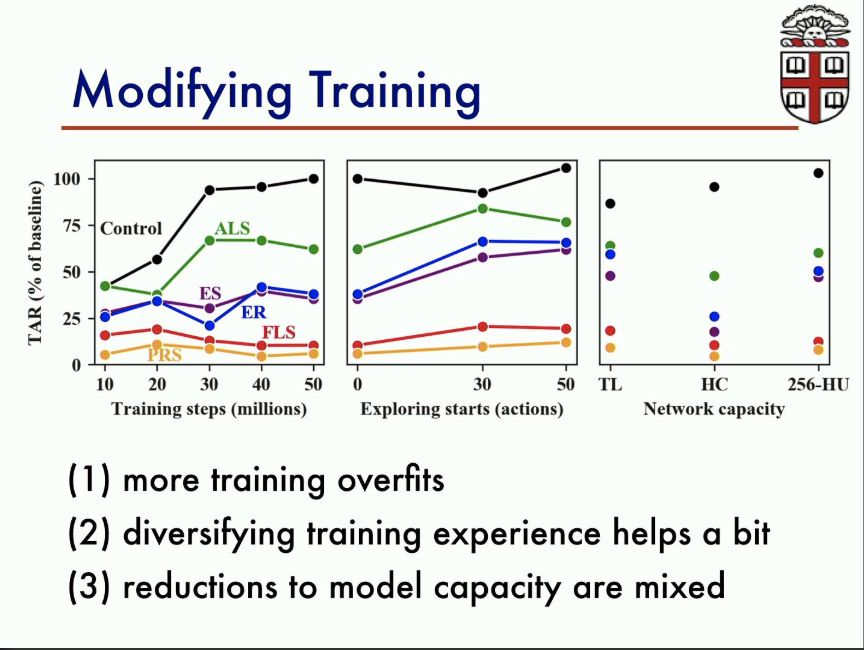
\includegraphics[width=0.7\textwidth]{figures/mod_train.png}
    \caption{Results for changing three aspects of training procedure}
    \label{fig:gen}
\end{figure}

Case Study: CoinRun \cite{cobbe2018quantifying}. New set of environments that are designed explicitly for studying generalization in RL.
\begin{itemize}
    \item Goal is to collect coin at the end of the level
    \item Agent spawns on the left
    \item Contains obstacles, enemies, level ends by death.
    \item Levels divided into three levels of difficulty.
    
    $\ra$ Results from \citet{cobbe2018quantifying} show {\it overfitting} curves, which is exciting to see in RL. See Figure \ref{fig:coinrun}.
\end{itemize}


\begin{figure}[h!]
    \centering
    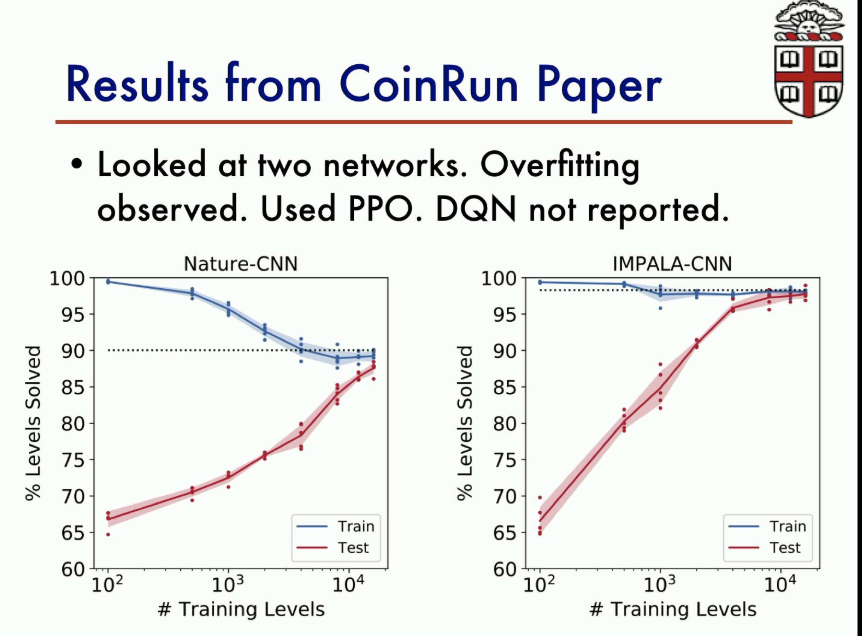
\includegraphics[width=0.7\textwidth]{figures/coin_run.png}
    \caption{Results on CoinRun domain from \citet{cobbe2018quantifying}}
    \label{fig:coinrun}
\end{figure}


But, the results on CoinRun were using a policy optimization method rather than DQN. \\

$\ra$ Tried to replicate with DQN, found the opposite result: it didn't work! Contacted the authors and they had found the same thing. \\

$\ra$ Later finding: DQN (and PPO) will generalize well with a lot of levels used (when the hard levels are removed). \\

Also studied prediction errors;
\begin{itemize}
    \item High prediction error associated with failure.
    \item Prediction error lower in training than testing.
    \item Training performance = testing performance  given enough data
\end{itemize}

Summary:
\begin{itemize}
    \item Good RL performance is seductive, but we need to look closer
    
    \item Analogy between RL and supervised learning is subtle
    \item DQN does not generalize well in Amidar, CoinRun, and some weak generalization in CoinRun difficulty 2.
    \item Found prediction error and internal representation 
    distance good predictors of poor generalization
    
    \item Adjusting training volume, model capacity, and exploration help, but only a bit.
\end{itemize}

\spacerule




% --- Bibliography ---
\newpage
\bibliographystyle{plainnat}
\bibliography{neurips}

\end{document}
